% body.tex
\newcommand{\bq}{}
\newcommand{\dpic}{{\bq dpic}\xspace}
\newcommand{\Dpic}{{\bq Dpic}\xspace}
\newcommand{\dvips}{{\bq dvips}\xspace}
\newcommand{\gpic}{{\bq gpic}\xspace}
\newcommand{\Gpic}{{\bq Gpic}\xspace}
\newcommand{\groff}{{\bq groff}\xspace}
\newcommand{\latex}{\LaTeX\xspace}
\newcommand{\linespec}{{\sl linespec}\xspace}
\newcommand{\MetaPost}{{\bq MetaPost}\xspace}
\newcommand{\Mfour}{{\bq m4}\xspace}
\newcommand{\mfpic}{{\bq mfpic}\xspace}
\newcommand{\PDF}{{\bq PDF}\xspace}
\newcommand{\pic}{{\bq pic}\xspace}
\newcommand{\Pic}{{\bq Pic}\xspace}
\newcommand{\Postscript}{{\bq Postscript}\xspace}
\newcommand{\PSTricks}{{\bq PSTricks}\xspace}
\newcommand{\SVG}{{\bq SVG}\xspace}
\newcommand{\tex}{\TeX\xspace}
\newcommand{\Textregistered}{\textregistered\xspace}
\newcommand{\TPGF}{{\bq Ti{\it k}z~PGF}\xspace}
\newcommand{\Tikz}{{\bq Ti{\it k}z}\xspace}
\newcommand{\tpic}{{\bq tpic}\xspace}
\newcommand{\xfig}{{\bq xfig}\xspace}
\newcommand{\Xfig}{{\bq Xfig}\xspace}
%
\newcommand{\xection}[1]{\section[\texorpdfstring{#1\ \dotfill}{#1}]{#1}}
\newcommand{\NVL}{\\\hspace*{\parindent}}
\newcommand{\brtt}{\hfill\break\hspace*\parindent}
\newcommand{\lbr}{{\tt\char123}}
\newcommand{\rbr}{{\tt\char125}}
\newcommand{\bsl}{{\tt\char92}}
\newcommand{\SR}[1]{\hyperref[#1]{Section~\ref*{#1}}}
\newcommand{\PR}[1]{\hyperref[#1]{page~\pageref*{#1}}}
\newcommand{\FR}[1]{\hyperref[#1]{Figure~\ref*{#1}}}
\newcommand{\FRS}[1]{\hyperref[#1]{Figures~\ref*{#1}}}
\newcommand{\REF}[1]{\hyperref[#1]{\ref*{#1}}}
\newcommand{\LQ}{\char96}
\newcommand{\RQ}{\char39}
%
\newcommand{\Example}[1]{\vspace{\parsep}\noindent {\bf Example #1:}}
%
%  \pdfbookmark[section]{\contentsname}{toc}
%\begin{multicols}{2}
%  \tableofcontents
%\end{multicols}
%
\xection{Introduction\label{Introduction:}}
   \begin{quotation}\noindent
   It appears that people
   who are unable to execute pretty pictures with pen and paper find it
   gratifying to try with a computer~\cite{Landauer95}.
   \end{quotation}

This manual%
\footnote{This document is best displayed with a reader that shows bookmarks.}
describes a method for drawing electric circuits and
other diagrams in \latex and web documents.
The diagrams are defined in the simple \pic drawing language~\cite{KRpic}
augmented with \Mfour macros~\cite{KRm4}, and are
processed by \Mfour and a \pic processor to
convert them to \TPGF, \PSTricks, other \latex-compatible code, or \SVG.
In its basic form, the method has the advantages and disadvantages of
\tex itself, since it is macro-based and non-WYSIWYG,
with ordinary text input.  The book from which the above quotation
is taken correctly points out that the payoff can be in quality of
diagrams at the price of the time spent in learning how to draw them.

A collection of basic components, most based on IEC and IEEE
standards~\cite{IECstd,IEEEstd},
and conventions for their internal
structure are described.  Macros such as these are only a starting
point, since it is often convenient to customize elements or to package
combinations of them for particular drawings.

\xection{Using the macros\label{Using:}}
This section describes the basic process of adding circuit diagrams to
\latex documents to produce postscript or pdf files.  On some operating
systems, project management software with graphical interfaces can
automate the process, but the steps can also be performed by a script,
makefile, or by hand for simple documents as described in~\SR{Quickstart:}.

The diagram source file is preprocessed as illustrated in
\FR{Flowdiag}.  A configuration file is read by \Mfour,
followed by the diagram source.
The result is passed through a
\pic interpreter to produce {\tt .tex} output that can be inserted
into a {\tt .tex} document using the \verb|\input| command.

\begin{figure}[ht]
 \pdftooltip{\input Flowdiag }{Flow diagram for the inclusion of figures}
 \caption{Inclusion of figures and macros in the \latex document.
 \label{Flowdiag}}
 \end{figure}

\noindent
The interpreter output contains
\TPGF~\cite{tikz} commands,
\PSTricks~\cite{pstricks} commands,
basic \latex graphics, 
\tpic specials, or other formats,
depending on the chosen options.
These variations are described in \SR{Alternative:}.

There are two principal choices of \pic interpreter.  One is~\dpic,
described later in this document.  A partial alternative is
GNU {\bq gpic -t} (sometimes simply named \pic)~\cite{gpic}
together with a printer driver
that understands \tpic specials, typically {\bq dvips}~\cite{dvips}.
The \dpic processor extends the pic language in small but important ways;
consequently, some of the macros and examples in this distribution work fully
only with \dpic.
\Pic processors contain basic macro facilities, so some of the
concepts applied here do not require \Mfour.

\subsection{Quick start\label{Quickstart:}}
The contents of file {\tt quick.m4} and resulting diagram are shown in
\FR{quick} to illustrate the language
% to show several ways for placing circuit elements,
%and to provide sufficient information for producing
and the production of basic labeled circuits.
\begin{figure}[h!]
   \parbox{\textwidth}{\small\verbatiminput{quick.m4}}%
   \hfill\llap{\raise-1.15in\hbox{\input quick }}%
%  \hfill\llap{\raise-1.15in\hbox{\pdftooltip{\input quick }%
%  {The file {\tt quick.m4} and resulting diagram.
%    There are several ways of drawing the same picture; for example,
%     nodes (such as {\tt Origin}) can be defined and circuit branches
%     drawn between them; or absolute coordinates can be used (e.g.,
%     {\tt source(up\_ from (0,0) to (0,0.75))} ).  Element sizes and styles
%     can be varied as described in later sections.}}}%
   \vspace*{-\baselineskip}%
   \caption{The file {\tt quick.m4} and resulting diagram.
     There are several ways of drawing the same picture; for example,
      nodes (such as {\tt Origin}) can be defined and circuit branches
      drawn between them; or absolute coordinates can be used (e.g.,
      {\tt source(up\_ from (0,0) to (0,0.75))} ).  Element sizes and styles
      can be varied as described in later sections.\label{quick}}%
   \end{figure}

\subsubsection{\protect{Using \Mfour}%
\label{Usingmfour:}}
The command

  {\vspace*\parsep\tt
    m4 {\sl filename \ldots}
   \vspace*\parsep}

\noindent
causes \Mfour\ to search for the named
files in the current directory and directories specified
by environmental variable {\tt M4PATH}. 
Set {\tt M4PATH} to the full name (i.e., the path) of the directory containing
{\tt libcct.m4} and the other circuit library {\tt .m4} files; otherwise
invoke \Mfour\ as {\tt m4 -I} {\sl installdir} 
where {\sl installdir} is the path to the directory
containing the library files.
Now there are at least two basic possibilities as follows,
but be sure to read \SR{Simplifications:} for simplified use.

\subsubsection{\protect{Processing with \dpic and \PSTricks or \TPGF}%
\label{Processingwithpstricks:}}
If you are using \dpic  with \PSTricks,
put \verb|\usepackage{pstricks}| in the main \latex source file header and
type the following commands or put them into a script:

  {\vspace*\parsep\tt
    m4 pstricks.m4 quick.m4 > quick.pic
    \brtt
    dpic -p quick.pic > quick.tex
   \vspace*\parsep}


\noindent
To produce \TPGF code,
the \latex header should contain \verb|\usepackage{tikz}|.
The commands are modified to read \verb|pgf.m4|
and invoke the {\tt-g} option of \dpic as follows:

  {\vspace*\parsep\tt
% {\tt
  m4 pgf.m4 quick.m4 > quick.pic
    \brtt
  dpic -g quick.pic > quick.tex
   \vspace*\parsep}
 
A configuration file ({\tt pstricks.m4} and {\tt pgf.m4} in the
above examples) is {\em always} the first file to be given to \Mfour.
Put the following or its equivalent in the document body:
\begin{verbatim}
\begin{figure}[ht]
   \centering
   \input quick
   \caption{Customized caption for the figure.}
   \label{Symbolic_label}
\end{figure}
\end{verbatim}
Then for \PSTricks,
the commands ``{\tt latex} {\sl file}{\tt;} {\tt dvips} {\sl file}''
produce {\sl file}{\tt.ps},
which can be printed or viewed using {\tt gsview}, for example.
For \TPGF,
Invoking PDFlatex on the source produces {\tt .pdf} output directly.
The essential line is \verb|\input quick| whether or not the figure
environment is used.

The effect of the \Mfour command above is shown in \FR{ConfigA}. 
Configuration files {\tt pstricks.m4} or {\tt pgf.m4}
cause library {\tt libgen.m4}
to be read, thereby defining the macro {\tt cct\_init}.
The diagram source file is then read and
the circuit-element macros in {\tt libcct.m4} are defined during
expansion of {\tt cct\_init}.
\begin{figure}[ht]
   \input ConfigA
   \caption{The command
     {\tt m4 pstricks.m4 quick.m4 > quick.pic}.
   \label{ConfigA}}
   \end{figure}

\subsubsection{Processing with \gpic\label{Processingwithgpic:}}
If your printer driver understands \tpic specials and
you are using \gpic  (on some systems the \gpic command is {\tt pic}),
the commands are

  {\tt
  m4 gpic.m4 quick.m4 > quick.pic
    \brtt
  gpic -t quick.pic > quick.tex
   \vspace*\parsep}

\noindent
and the figure inclusion statements are as shown:
\begin{verbatim}
\begin{figure}[ht]
   \input quick
   \centerline{\box\graph}
   \caption{Customized caption for the figure.}
   \label{Symbolic_label}
   \end{figure}
\end{verbatim}

\subsubsection{Simplifications\label{Simplifications:}}
M4 must read a configuration file before any other files,
%followed by the macro definitions in one or more library files,
either before reading the diagram source file or at the beginning of it.
There are several ways to control the process, as follows:
\begin{enumerate}
\item
The macros can be processed by \latex-specific
project software and by graphic applications such as
Pycirkuit~\cite{Mas2019}.
% Cirkuit~\cite{KDEApps2009}.
Alternatively when many files are to be processed, a facility such as
Unix ``make,'' which is also available in PC and Mac versions, can be employed
to automate the required commands.  On systems without such
facilities, a scripting language can be used.

\item
The \Mfour commands illustrated above can be shortened to

\verb|m4 quick.m4 > quick.pic|

\noindent
by inserting {\tt include(pstricks.m4)} (assuming \PSTricks processing)
%or {\tt include(libgen.m4)} (assuming the default processor is to be used)
{\em immediately} after the {\tt .PS} line, the effect of which 
%The effect of the first include statement
is shown in \FR{ConfigB}.
However, if you then want to use \TPGF,
the line must be changed to {\tt include(pgf.m4)}.
%and the second in \FR{ConfigC}.
\begin{figure}[h!]
   \input{ConfigB}
   \caption{The command {\tt m4 quick.m4 > quick.pic},
   with {\tt include(pstricks.m4)} preceding {\tt cct\_init}.}
   \label{ConfigB}
   \end{figure}
%\begin{figure}[h!]
%   \input{ConfigC}
%   \caption{The command {\tt m4 quick.m4 > quick.pic},
%   with {\tt include(libgen.m4)} preceding {\tt cct\_init}, causing
%   the default configuration file to be read.}
%   \label{ConfigC}
%   \end{figure}

%\item
%On some systems, setting the environment variable {\tt M4PATH} to {\sl
%installdir} allows the {\tt -I} {\sl installdir} option of \Mfour to
%be omitted, but it will be kept in following examples.

\item
In the absence of a need to examine the file {\tt quick.pic},
the commands for producing the {\tt .tex} file can be reduced
(provided the above inclusions have been made) to

\verb%m4 quick.m4 | dpic -p > quick.tex%

\enlargethispage{\baselineskip}
\item
You can put several diagrams into a single source file.
Make each diagram the body of a \latex macro, as shown:

\par
\verb|\newcommand{\diaA}{%|\NVL
\verb|.PS|\NVL
{\sl drawing commands}\NVL
\verb|.PE|\NVL
\verb|\box\graph }%  \box\graph not required for dpic|\NVL
\verb|\newcommand{\diaB}{%|\NVL
\verb|.PS|\NVL
{\sl drawing commands}\NVL
\verb|.PE|\NVL
\verb|\box\graph }%  \box\graph not required for dpic|\NVL
Produce a {\tt .tex} file as usual,
insert the {\tt .tex} into the \latex source, and
invoke the macros \verb^\diaA^ and \verb^\diaB^ at the appropriate places.

\item
%Whether this and the next item rightly belong under the heading
%``Simplifications'' might be debated. They appear most useful
%when a project-management tool is employed.
In some circumstances,
it may be desirable to invoke \Mfour and \dpic automatically from the
document. Define a macro \verb|\mtotex| as shown in the
following example:

{\tt \verb^\documentclass{article}^ \brtt
\verb^\usepackage{tikz}^ \brtt
\verb^\newcommand\mtotex[2]{\immediate\write18{m4 ^%-I^ {\sl installdir}
\verb^#2.m4 | dpic -#1 > #2.tex}}%^\break
\verb^\begin{document}^ \brtt
\verb^\mtotex{g}{FileA} % Generate FileA.tex^ \brtt
\verb^\input{FileA.tex} \par^ \brtt
\verb^\mtotex{g}{FileB} % Generate FileB.tex^ \brtt
\verb^\input{FileB.tex}^ \brtt
\verb^\end{document}^
   \vspace*\parsep}

The first argument of \verb|\mtotex| is a {\tt p} for pstricks or
{\tt g} for pgf.
Sources \verb|FileA.m4| and \verb|FileB.m4| must contain any required
\verb|include| statements,
and the main document should be processed using
the latex or pdflatex option \verb|--shell-escape|.
If the {\tt M4PATH} environment variable is not set then insert
{\tt -I }{\sl installdir} after {\tt m4} in the command definition,
where {\sl installdir} is the absolute path to the installation directory.
This method processes the picture source each time \latex is run, so for
large documents containing many diagrams, the \verb|\mtotex|
lines could be commented out after debugging the corresponding graphic.
A derivative of this method that allows the insertion of
\pic code into a \Tikz picture is described in \SR{Tikzwithpic:}.

\item
It might be convenient for the source of small diagrams to be part
of the document source text.  The {\tt filecontents} environment of current
\LaTeX\ allows this; older versions can employ a now-obsolete package
{\tt filecontents.sty}.  The following example
for processing by {\tt pdflatex} \verb|--shell-escape|
first writes the \Mfour\ source
to file {\tt sample.m4}, invokes \verb|\mtotex| on it, and reads in the result:

\par
\verb|\begin{filecontents}[overwrite,noheader,nosearch]{sample.m4}|\NVL
\verb|include(pgf.m4)|\NVL
\verb|.PS|\NVL
\verb|cct_init|\NVL
{\sl drawing commands} $\ldots$\NVL
\verb|.PE|\NVL
\verb|\end{filecontents}|\NVL
\verb|\mtotex{g}{sample}|\NVL
\verb|\documentclass{article}
\usepackage[dvipdfm]{graphicx}
\usepackage[dvipdfm]{color}
\usepackage[dvipdfm]{hyperref}
\title{\color{blue}Latex Support Test File}
\author{\color{green}Mark A. Wicks}
\begin{document}
\maketitle
\section{Introduction}
This document is primarily intended
to demonstrate the functionality
of some \LaTeX packages that require
driver support for their functionality.
It is quick-and-dirty.
It is not intended to be pretty, and
does not demonstrate good ways to use these packages
(In fact, it demonstrates some bad ways to use these packages).

\section{Driver Files}
This distribution of {\tt dvipdfm} includes
the {\tt .def} files required to support
the \textcolor{green}{color},
\rotatebox{30}{\textcolor{red}{graphics}}, and hyperref \LaTeX\space
packages.  Once these .def files
are installed where these packages
can find them.  You also may need
to modify {\tt color.sty}, {\tt graphics.sty},
and {\tt hyperref.sty} so that they
recognize {\tt dvipdfm} as a driver.
Once these {\tt .def} files are installed,
you should be able to use {\tt dvipdfm}
with \LaTeX for many applications.

After running \LaTeX on this
document, {\tt hyperref}
should produce a hyperlinked
document, complete with an outline.

\newpage
\section{Graphics Support}
Currently, JPEG and PDF image
inclusion are supported.

\subsection{JPEG Image Inclusion}
Figure~\ref{fig:author}
shows a photograph of the author
that was obtained from a JPEG file.
A small file with the extension of {\tt .bb}
supplies the bounding box to the \LaTeX\space
Graphics package.  For PDF and JPEG files,
this bounding box can easily be created by running
the {\tt ebb} utility included with this
distribution of {\tt dvipdfm}.

\begin{figure}
  \begin{center}
    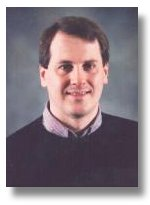
\includegraphics{mwicks.jpeg}
  \end{center}

  \caption{A photograph of the author.}
  \label{fig:author}
\end{figure}

\subsection{PDF Image Inclusion}
Figure~\ref{fig:circuit} shows
an electronics circuit,
drawn with XFig, distilled,
and then included as PDF file.
\begin{figure}
  \begin{center}
     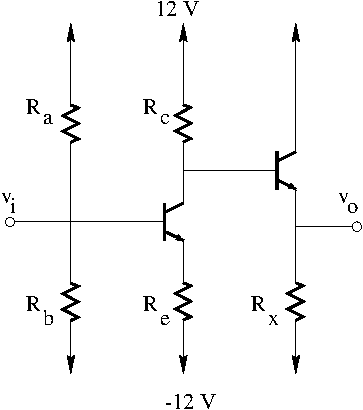
\includegraphics{transistor.pdf}
  \end{center}

  \caption{A simple two-stage transistor circuit.}
  \label{fig:circuit}
\end{figure}

\begin{figure}
  \begin{center}
     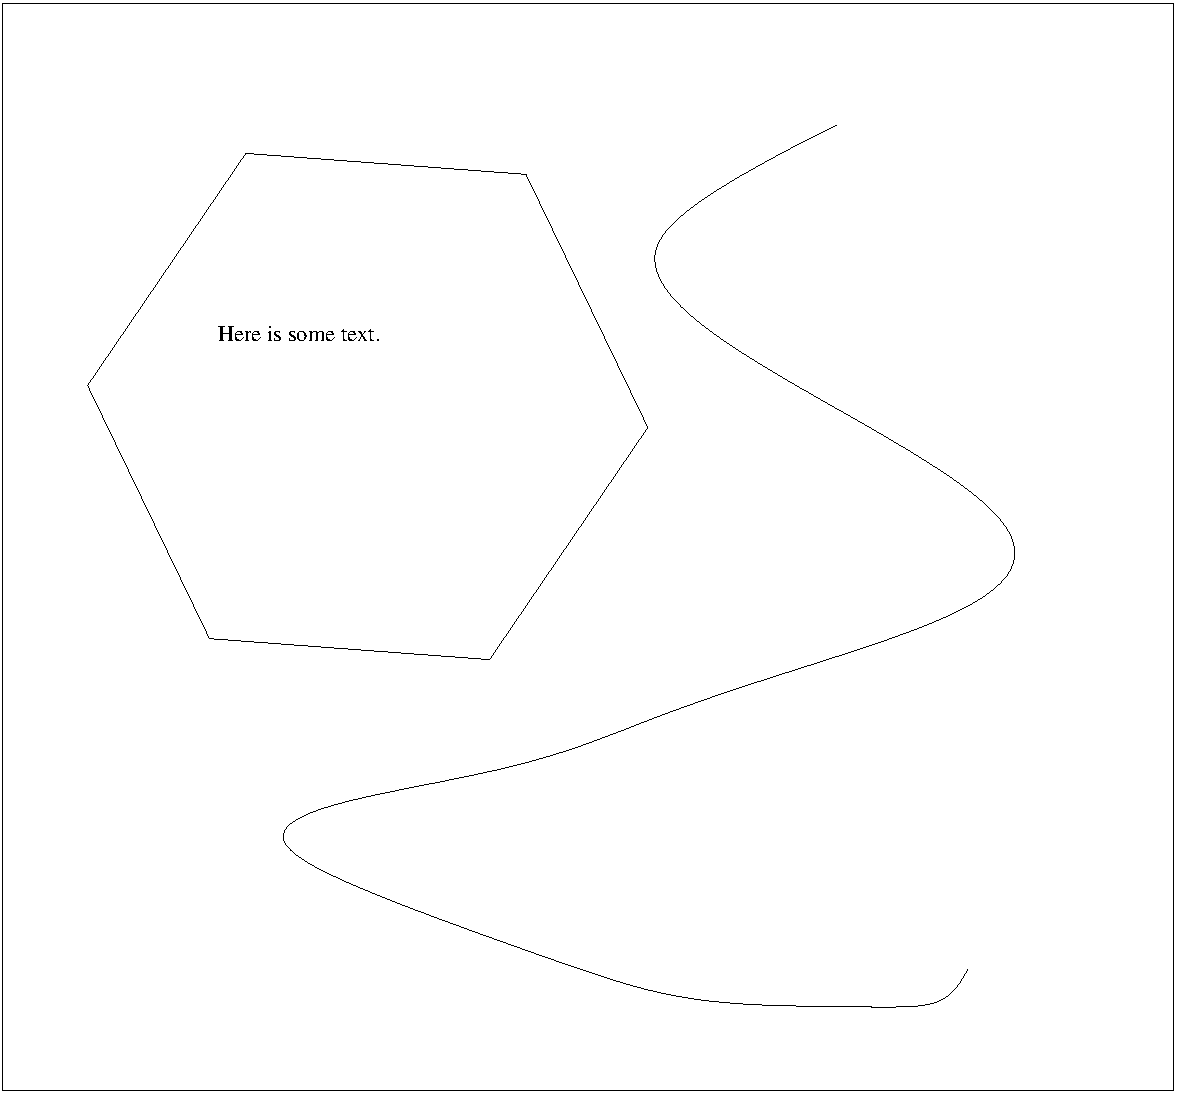
\includegraphics[width=3.0in]{something.pdf}
  \end{center}

  \caption{A second included figure}
  \label{fig:something}
\end{figure}

\end{document}
|\NVL
\end{enumerate}

\subsection{Including the libraries\label{Libraries:}}
The configuration files for \dpic are as follows,
depending on the output format (see \SR{Alternative:}):
{\tt pstricks.m4, pgf.m4, mfpic.m4, mpost.m4, postscript.m4, psfrag.m4, svg.m4,
 gpic.m4,} or {\tt xfig.m4}.
The file {\tt psfrag.m4} simply defines the macro {\tt psfrag\_} and
then reads {\tt postscript.m4}.
For \gpic, the configuration file is {\tt gpic.m4}.
The usual case for producing circuit diagrams is to read
{\tt pstricks.m4} or {\tt pgf.m4} first when \dpic is the postprocessor or
to set one of these as the default configuration file.

At the top of each diagram source, put one or more initialization
commands; that is,

{\tt cct\_init, log\_init, sfg\_init, darrow\_init, threeD\_init}

\noindent
or, for diagrams not requiring specialized macros, {\tt gen\_init}.
As shown in \FRS{ConfigA} and~\REF{ConfigB},
each initialization command reads in the appropriate macro
library if it hasn't already been read;
for example, {\tt cct\_init} tests whether {\tt libcct.m4} has been
read and includes it if necessary.

A few of the distributed example files contain other experimental macros
that can be pasted into diagram source files; see
{\tt Flow.m4} or {\tt Buttons.m4}, for example.

The libraries contain hints and explanations that might help in debugging
or if you wish to modify any of the macros.  Macros are generally named
using the obvious circuit element names so that programming becomes something
of an extension of the \pic language.  Some macro names end in an underscore
to reduce the chance of name clashes.  These can be invoked in the
diagram source but there is no long-term guarantee that their names and
functionality
will remain unchanged. Finally, macros intended only for internal use
begin with the characters {\tt m4}.

\xection{\Pic essentials\label{Pic:}}

\Pic source is a sequence of lines in a text file.
The first line of a diagram begins with {\tt .PS} with optional following
arguments, and the last line is normally {\tt .PE}.
Lines outside of these pass through the \pic processor unchanged.

The visible objects can be divided conveniently into two classes, the
{\em linear} objects {\tt line, arrow, spline, arc,} and the
{\em planar} objects {\tt box, circle, ellipse.}

The object {\tt move} is linear but draws nothing.  A compound object,
or {\tt block,} is planar and consists of a pair of square brackets enclosing
other objects, as described in \SR{Compoundobjects:}.

Objects can be placed using absolute coordinates or,
as is often better, relative to other objects.

\Pic allows the definition of real-valued variables, which are alphameric
names beginning with lower-case letters, and computations using them.
Objects or locations on the diagram can be given symbolic names
beginning with an upper-case letter.

\subsection{Manuals\label{Manuals:}}
The classic \pic manual~\cite{KRpic} is still a good introduction to \pic, but
a more complete manual~\cite{Raymond95} can be found in the GNU \groff\
package, and both are available on the web~\cite{KRpic,Raymond95}.  Reading
either will give you competence with \pic in an hour or two.  Explicit mention
of {\tt *roff} string and font constructs in these manuals should be replaced by
their equivalents in the \latex context.  A man-page language summary is
appended to the \dpic manual~\cite{Aplevich2011}.

A web search will yield good discussions of ``little languages'';
for \pic in particular, see Chapter~9 of~\cite{Bentley88}.
Chapter~1 of reference~\cite{Goossens97} also contains a brief
discussion of this and other languages.

\subsection{The linear objects: {\tt line, arrow, spline, arc}%
\label{Linearobjects:}}
A line can be drawn as follows:

{\tt line from} {\sl position} {\tt to} {\sl position}

\noindent
where {\sl position} is defined below or

{\tt line} {\sl direction} {\sl distance}

\noindent
where {\sl direction} is one of {\tt up,} {\tt down,} {\tt left,}
{\tt right.}  When used with the \Mfour macros described here, it is
preferable to add an underscore: {\tt up\_,} {\tt down\_,} {\tt left\_,}
{\tt right\_.}  The {\sl distance} is a number or expression
and the units are inches, but the assignment

{\tt scale = 25.4}

\noindent
has the effect of changing the units to millimetres,
as described in \SR{Scaling:}.

Lines can also be drawn to any distance in any direction.  The example,

{\tt line up\_ 3/sqrt(2) right\_ 3/sqrt(2) dashed}

\noindent
draws a line 3 units long from the current location,
at a $45^\circ$ angle above horizontal.
Lines (and other objects) can be specified as {\tt dotted,} {\tt dashed,} or
{\tt invisible,} as above.

The construction

{\tt line from A to B chop x}

\noindent
truncates the line at each end by {\tt x} (which may be negative)
or, if {\tt x} is omitted, by
the current circle radius, a convenience when A and B are
circular graph nodes, for example.  Otherwise

{\tt line from A to B chop x chop y}

\noindent
truncates the line by {\tt x} at the start and {\tt y} at the end.

Any of the above means of specifying line (or arrow) direction and length
will be called a \linespec.

Lines can be concatenated.  For example, to draw a triangle:

{\tt line up\_ sqrt(3) right\_ 1 then down\_ sqrt(3) right\_ 1 then left\_ 2}

\subsection{Positions\label{Positions:}}
A {\sl position} can be defined by a coordinate pair, e.g. {\tt 3,2.5},
more generally using parentheses by {\tt (}{\sl expression, expression}{\tt )},
as a sum or difference as
{\tt{\sl position} $+$ ({\sl expression, expression})},
or by the construction {\tt (}{\sl position, position}{\tt )},
the latter taking the $x$-coordinate from the first
position and the $y$-coordinate from the second.  A position can be
given a symbolic name beginning with an upper-case letter,
e.g. {\tt Top:~(0.5,4.5)}.  Such a definition does not affect the calculated
figure boundaries.  The current position {\tt Here} is always defined and
is equal to $(0,0)$ at the beginning of a diagram or block.
The coordinates of a position are accessible, e.g. {\tt Top.x} and
{\tt Top.y} can be used in expressions.  The center, start, and end of
linear objects (and the defined points of other objects as described below)
are predefined positions, as shown in the following example,
which also illustrates how to refer to a previously drawn element if it has
not been given a name:

{\tt line from last line.start to 2nd last arrow.end then to 3rd line.center}

Objects can be named (using a name commencing with an upper-case letter),
for example:

{\tt Bus23: line up right}

\noindent
after which, positions associated with the object can be referenced using the
name; for example:

{\tt arc cw from Bus23.start to Bus23.end with .center at Bus23.center}

An arc is drawn by specifying its rotation, starting point, end point, and
center, but sensible defaults are assumed if any of these are omitted.
Note that

{\tt arc cw from Bus23.start to Bus23.end}

\noindent
does {\em not} define the arc uniquely; there are two arcs that satisfy this
specification.
This distribution includes the \Mfour macros

{\tt arcr( {\sl position, radius, start radians, end radians, modifiers, ht})
\hfill\break\indent
     arcd( {\sl position, radius, start degrees, end degrees, modifiers, ht})
\hfill\break\indent
     arca( {\sl chord linespec,} ccw|cw, {\sl radius, modifiers})
}

\noindent to draw uniquely defined arcs.
If the fifth argument of {\tt arcr} or {\tt arcd} contains {\tt ->} or {\tt <-}
then a midpoint arrowhead of height specified by arg6 is added.
For example,

{\tt arcd((1,-1),{},0,-90,<- outlined "red") dotted}

\noindent draws a red dotted arc with midpoint arrowhead,
 centre at $(1,-1),$ and default radius.
 The example

{\tt arca(from (1,1) to (2,2),{,}1,->)}

\noindent draws an acute angled arc with arrowhead on the chord defined by the
first argument.

The linear objects can be given arrowheads at the start, end, or both ends,
for example:

{\tt line dashed <- right 0.5\hfill\break
\hspace*{\parindent}%
arc <-> height 0.06 width 0.03 ccw from Here to Here+(0.5,0)
 \char92\hfill\break
\hspace*{2\parindent}%
   with .center at Here+(0.25,0)\hfill\break
\hspace*{\parindent}%
spline -> right 0.5 then down 0.2 left 0.3 then right 0.4}

The arrowheads on the arc above have had their shape adjusted using the
{\tt height} and {\tt width} parameters.

\subsection{The planar objects: {\tt box, circle, ellipse}, and text%
\label{Planarobjects:}}
Planar objects are drawn by specifying the width, height, and position, thus:

{\tt A: box ht 0.6 wid 0.8 at (1,1)}

\noindent
after which, in this example, the position {\tt A.center} is defined,
and can be referenced simply as {\tt A}.
The compass points {\tt A.n,} {\tt A.s,} {\tt A.e,} {\tt A.w,} {\tt A.ne,}
{\tt A.se,} {\tt A.sw,} {\tt A.nw} are automatically defined, as are
the dimensions {\tt A.height} and {\tt A.width.}
Planar objects can also be placed by specifying the location of a defined
point; for example, two touching circles can be drawn as shown:

{\tt circle radius 0.2\hfill\break 
\hspace*{\parindent}%
circle diameter (last circle.width * 1.2) with .sw at last circle.ne}

The planar objects can be filled with gray or colour.
For example, either

{\tt box dashed fill\_({\sl number})}\quad or\quad
 {\tt box dashed outlined "{\sl color}" shaded "{\sl color}"}

\noindent
produces a dashed box. The first case has a gray fill determined by
{\sl number}, with $0$ corresponding to black and $1$ to white;
the second case allows color outline and fill, the color strings depending on
the postprocessor.
Postprocessor-compatible RGB color strings are produced by the macro
{\tt rgbstring({\sl red fraction, green fraction, blue fraction})};
to produce an orange fill for example:

{\tt ... shaded rgbstring( 1, 0.645, 0)}

Basic colours for lines and fills are provided by \gpic  and \dpic,
but more elaborate line and fill styles or other effects
can be incorporated, depending on the postprocessor, using
%by inserting postprocessor commands using
%{\tt \char92 special} commands or
%other lines beginning with a backslash in the drawing code.  In fact,
%arbitrary lines can be inserted into the output using

{\tt command "}{\sl string}{\tt "}

\noindent where {\sl string} is one or more postprocessor command lines.

Arbitrary text strings, typically meant to be typeset by \latex, are
delimited by double-quote characters and occur in two ways.  The first
way is illustrated by

\verb|"\large Resonances of $C_{20}H_{42}$"|
 \verb|wid |{\sl x}\verb| ht |{\sl y}\verb| at |{\sl position}

\noindent
which writes the typeset result, like a box, at {\sl position} and tells
\pic its size.  The default size assumed by \pic is given by parameters
{\tt textwid} and {\tt textht} if it is not specified as above.
The exact typeset size of formatted text can be obtained
as described in \SR{Interaction:}.  The second occurrence
associates one or more strings with an object, e.g., the following writes
two words, one above the other, at the centre of an ellipse:

\verb|ellipse "\bf Stop" "\bf here"|

\noindent
The C-like \pic function
 {\tt sprintf("{\sl format string}",{\sl numerical arguments})}
is equivalent to a string.

\subsection{Compound objects\label{Compoundobjects:}}
A compound object is a group of statements enclosed in square
brackets.  Such an object is placed by default as if it were a box, but
it can also be placed by specifying the final position of a defined point.
A defined point is the center or compass corner of the bounding box
of the compound object or one of its internal objects.
Consider the last line of the code fragment shown:

\noindent%
\verb|  Ands: [ right_|\\
\verb|          And1: AND_gate|\\
\verb|          And2: AND_gate at And1 - (0,And1.ht*3/2)|\\
\verb|          |$\ldots$\\
\verb|        ] with .And2.In1 at| {\sl position} % (K.x,IC5.Pin9.y)|

The two gate macros evaluate to compound objects containing {\tt Out},
{\tt In1}, and other locations.  The final positions of all objects
inside the square brackets are determined in the last line by
specifying the position of {\tt In1} of gate {\tt And2}.

\subsection{Other language facilities\label{Otherlanguage:}}

All objects have default sizes, directions, and other characteristics,
so part of the specification of an object can sometimes be profitably
omitted.

Another possibility for defining positions is 

{\sl expression} {\tt between} {\sl position}
 {\tt and} {\sl position}

\noindent%
which means 

$\hbox{\sl 1st position} + \hbox{\sl expression} \times 
  (\hbox{\sl 2nd position} - \hbox{\sl 1st position})$

\noindent and which can be abbreviated as

{\sl expression} {\tt <} {\sl position} {\tt ,} {\sl position} {\tt >}

\noindent%
Care has to be used in processing the latter construction with \Mfour,
since the comma may have to be put within quotes, {\tt `,'}
to distinguish it from the {\tt m4} argument separator.

Positions can be calculated using expressions containing variables.
The scope of a position is the current block.  Thus, for example,

{\tt
  theta = atan2(B.y-A.y,B.x-A.x)

  line to Here+(3*cos(theta),3*sin(theta)).
  }

Expressions are the usual algebraic combinations of primary quantities:
constants, environmental parameters such as {\tt scale,} variables,
horizontal or vertical coordinates of terms such as
{\sl position}{\tt.x} or {\sl position}{\tt.y},
dimensions of \pic objects, e.g. {\tt last circle.rad}.
The elementary algebraic operators are
{\tt +, -, *, /, \%, =, +=, -=, *=, /=,} and {\tt \%=,}
similar to the C language.

The logical operators {\tt ==, !=, <=, >=, >,} and {\tt <} apply to
expressions and strings.  A modest selection of numerical functions is
also provided: the single-argument functions {\tt sin, cos, log, exp,
sqrt, int}, where {\tt log} and {\tt exp} are base-10, the two-argument
functions {\tt atan2, max, min,} and the random-number generator {\tt
rand()}.  Other functions are also provided using macros.

A \pic manual should be consulted for details, more examples, and
other facilities, such as the branching facility

\verb|if |{\sl expression}\verb| then { |{\sl anything} 
  \verb|} else { |{\sl anything}\verb| }|,

\noindent%
the looping facility

\verb|for |{\sl variable}\verb| = |{\sl expression}\verb| to |% 
{\sl expression}\verb| by |{\sl expression}\verb| do { |%
{\sl anything}\verb| }|,

\noindent%
operating-system commands, \pic macros, and external file inclusion.

\xection{Two-terminal circuit elements\label{Basictwo:}}
There is a fundamental difference between the two-terminal elements, each
of which is drawn along an invisible straight-line segment,
and other elements, which are compound objects mentioned
in \SR{Compoundobjects:}.
% Specifying the straight-line segment requires four numbers, the coordinates
% of the start and end, or equivalent, but default values are used if
% not specified.
The two-terminal element macros follow a
set of conventions described in this section, and other elements will
be described in \SR{Composite:}.

\subsection{Circuit and element basics\label{Basics:}}
A list of the library macros and their arguments is in
\SR{defines}.  The arguments have default values, so that only
those that differ from defaults need be specified.

\FR{BigResistor}, which shows a resistor, also serves as
an example of \pic commands.
%Consider the resistor shown in \FR{BigResistor},
%which also serves as an example of \pic commands.
The first part of the source file for this figure is 
%as follows:
on the left:

\begin{figure}[ht]
   \parbox{2in}{\tt .PS\\ \hbox{}\quad cct\_init\\ \hbox{}\quad linewid = 2.0\\ 
     \hbox{}\quad linethick\_(2.0)\\ R1: resistor}
   \raisebox{-0.3in}{\hbox{\input{BigResistor.tex}}}
   \caption{Resistor named {\tt R1}, showing the size parameters,
     enclosing block, and predefined positions.}
   \label{BigResistor}
   \end{figure}
The lines of \FR{BigResistor}
and the remaining source lines of the file are explained below:
\begin{itemize}
\item The first line invokes the macro {\tt cct\_init} that
   loads the library {\tt libcct.m4} 
   and initializes local variables needed by some circuit-element macros.

\item
   The sizes of circuit elements are proportional to the \pic environmental
   variable {\tt linewid}, so redefining this variable changes element
   sizes.  The element body is drawn in proportion to {\tt dimen\_},
   a macro that evaluates to {\tt linewid} unless redefined, and the default
   element length is {\tt elen\_}, which evaluates to
   {\tt dimen\_*3/2} unless redefined.
   Setting {\tt linewid} to 2.0 as in the example means that the default element
   length becomes 3.0\,in.
   For resistors, the default length of the body is {\tt dimen\_/2,} and the
   width is {\tt dimen\_/6.} All of these values can be customized.
   Element scaling and the use of SI units is discussed further in
   \SR{Scaling:}.

\item The macro {\tt linethick\_} sets the default thickness of subsequent
   lines (to 2.0\,pt in the example).
   Macro arguments are written within parentheses
   following the macro name, with no space between the name and the
   opening parenthesis.  Lines can be broken before macro arguments
   because \Mfour and \dpic ignore white space immediately preceding
   arguments.  Otherwise, a long line can be continued to the next
   by putting a backslash as the rightmost character. 
\item The two-terminal element macros expand to sequences of drawing commands
   that begin with {\tt `line invis \linespec'},
   where \linespec is the first argument of the macro if it
   is non-blank, otherwise the line is drawn a distance
   {\tt elen\_} in the current direction, which is to the right by
   default.
%  All this is handled by the macro {\tt eleminit\_}, which also
%  calculates the length and angle of the invisible line for later use.
   The invisible line is first drawn, then the element is drawn
   on top of it.
   The element---rather, the initial invisible line---can
   be given a name, {\tt R1} in the example, so that positions
   {\tt R1.start}, {\tt R1.centre}, and {\tt R1.end} are automatically
   defined as shown.
\item The element body is overlaid by a block, which can be
   used to place labels around the element.  The block
   corresponds to an invisible rectangle with horizontal top and bottom lines,
   regardless of the direction in which the element is drawn.  A
   dotted box has been drawn in the diagram to show the block boundaries.
\item The last sub-element, identical to the first in two-terminal
   elements, is an invisible line that can be referenced later to
   place labels or other elements.
%  This might be over-kill.
   If you create your own macros, you might choose simplicity over generality,
   and include only visible lines.
  \end{itemize}

To produce \FR{BigResistor}, the following embellishments
were added after the previously shown source:
{\small \input BigResistor2.verb }

\begin{itemize}
\item The line thickness is set to the default thin value of \hbox{0.4\,pt},
   and the box displaying the element body block is drawn.  Notice how the
   width and height can be specified, and the box centre positioned at
   the centre of the block.
\item The next paragraph draws two objects, a spline with an arrowhead,
   and a string left justified at the end of the spline.  Other
   string-positioning modifiers than {\tt ljust} are {\tt rjust,}
   {\tt above,} and {\tt below.}

\item The last paragraph invokes a macro for dimensioning diagrams.
   \end{itemize}

\subsection{The two-terminal elements\label{Twoterminal:}}
The two-terminal elements are shown in
\FRS{Resistors} 
to~\REF{Switches} and part of~\FR{Arresters}.
Several elements are included more than once to illustrate
some of their arguments, which are listed in detail in \SR{defines}.
\FR{Resistors} shows some resistors with typical variants.
\begin{figure}[h!]
   \input ResistorsMan
   \caption{Resistors dawn by the macro
   {\tt resistor({\sl linespec, n}|E, {\sl chars}, {\sl cycle wid})}.
   The second argument is either an integer to specify number of cycles,
   the letter {\tt E}, or blank. The third argument specifies the desired
   variant.
   The default {\tt ebox} element designates a resistor.}
   \label{Resistors}
    \end{figure}

The first macro argument specifies
the invisible line segment along which the element is drawn.
If the argument is blank,
the element is drawn from the current position in the current drawing
direction along a default length.
The other arguments produce variants of the default elements.

Thus, for example,
\par
{\tt resistor(up\_ 1.25,7)}
\par
\noindent%
draws a resistor 1.25 units long up from the current position, with $7$
vertices per side.
The macro {\tt up\_} evaluates to {\tt up} but also resets the current
directional parameters to point up.

\pagebreak
Capacitors are illustrated in \FR{Capacitors}.
See \SR{Composite:} for the {\tt variable} macro.
\begin{figure}[h!t]
   \input CapacitorsMan
   \caption{The {\tt capacitor({\sl linespec, chars,} [R],{\sl height, width})}
      macro, and an example application of the {\tt variable} macro.}
   \label{Capacitors}
    \end{figure}

Basic inductors are illustrated in \FR{Inductors}.
\begin{figure}[h!]
   \input InductorsMan
   \caption{Basic inductors created with the
    {\tt inductor({\sl linespec,} W|L, {\sl cycles,} M|P|K, {\sl loop wid})}
    macro, the {\tt ebox} macro for European-style inductors, and some
    modifications (see also \SR{Composite:}).
    When an embellished element is repeated several times,
    writing a wrapper macro may be desirable.}
   \label{Inductors}
    \end{figure}

Some more basic elements are in \FR{MoreTable}, and amplifiers in \FR{AmpTable}.
\begin{figure}[h!t]
   \input MoreTableMan
   \caption{More two-terminal elements.}
   \label{MoreTable}
    \end{figure}
\begin{figure}[h!t]
   \input AmpTableMan
   \caption{Amplifier, delay, and integrator.}
   \label{AmpTable}
   \end{figure}

\FR{Sources} shows sources, many of which contain internal symbols,
and of which the {\tt AC} and {\tt S} options illustrate the need
to draw a single cycle of a sinusoid or approximate sinusoid.
\begin{figure}[h!t]
   \input SourcesMan
   \caption{Sources and source-like elements.}
   \label{Sources}
   \end{figure}
As a convenience,
the macro {\tt ACsymbol(at {\sl position, length, height,}
  [A]U|D|L|R|{\sl degrees})} is included as an interface to
the {\tt sinusoid} macro.  For example to add the sumbol
``\input{ACsymbol.tex}'' to an ebox:
\par
{\tt ebox; $\lbrace$\ ACsymbol(at last [],{,},dimen\_/8) $\rbrace$}

\noindent
For direct current (\input{DCsymbol.tex}), there is also
{\tt DCsymbol(at {\sl position, length, height,} U|D|L|R|{\sl degrees})},
and for power-system diagrams, macros
{\tt Deltasymbol(at {\sl position, keys,} U|D|L|R|{\sl degrees})},
and
{\tt Ysymbol(at {\sl position, keys,} U|D|L|R|{\sl degrees})},

\pagebreak
Diodes and fuses are shown in \FRS{Diodes} and \REF{Fuses}.
\begin{figure}[h!]
   \input DiodesMan
   \caption{The macro
     {\tt diode(\linespec,B|CR|D|L|LE[R]|P[R]|S|T|V|v|w|Z|{\sl chars},[R][E])}.
      Appending {\tt K} to the second argument draws an open arrowhead.}
   \label{Diodes}
   \end{figure}
\begin{figure}[h!]
   \input FusesMan
   \caption{Variations of the macros
     {\tt fuse(\linespec, A|dA|B|C|D|E|S|HB|HC|SB, {\sl wid}, {\sl ht})}
     and {\tt cbreaker(\linespec,L|R,D|T|TS)}.}
   \label{Fuses}
   \end{figure}

\enlargethispage{\baselineskip}%
Most of the two-terminal elements are oriented; that is, they have
a defined direction or polarity.  Several element macros include an
argument that reverses polarity, but there is also a more general
mechanism, as follows.

The first argument of the macro
\par
{\tt reversed(`}{\sl macro name}{\tt',}{\sl macro arguments}{\tt )}
\par
\noindent
is the name of a two-terminal element in quotes, followed by the
element arguments.  The element is drawn with reversed direction; thus,
\par
{\tt diode(right\_ 0.4); reversed(`diode',right\_ 0.4)}
\par
\noindent
draws two diodes to the right, but the second one points left.

Similarly, the macro
\par
{\tt resized(}{\sl factor},`{\sl macro name}',{\sl macro arguments}{\tt )}
\par
\noindent
can be used to resize the body of an element by temporarily multiplying
the {\tt dimen\_} macro by {\sl factor}. More general resizing should be
done by redefining {\tt dimen\_} as described in \SR{Circuitscaling:}.
These two macros can be nested; the following scales the above example
by 1.8, for example
\par
{\tt resized(1.8,`diode',right\_ 0.4);}
{\tt resized(1.8,`reversed',`diode',right\_ 0.4)}

\FR{Emarrows} contains radiation-effect arrows for embellishing two-terminal
and other macros.
\begin{figure}[h!]
   \input EmarrowsMan
   \caption{Radiation arrows: {\tt em\_arrows({\sl type, angle, length})}}
   \label{Emarrows}
   \end{figure}
The arrow stems are named {\sl A1}, {\sl A2},
and each pair is drawn in a \verb|[]| block, with
the names {\sl Head} and {\sl Tail} defined to
aid placement near another device.  The second argument specifies
absolute angle in degrees (default 135 degrees).
The arrows are drawn relative to the diode direction by the {\tt LE}
option in \FR{Diodes}.  For absolute arrow directions, one can
define a wrapper (see \SR{Writing:}) for the {\tt diode} macro to draw arrows
at 45 degrees, for example:
\par
{\tt define(`myLED',`diode(`\$1'); em\_arrows(N,45)
 with .Tail at last [].ne')}

\enlargethispage{\baselineskip}
Switches with numerous controls are in \FR{Switches}.
\begin{figure}[h!]
   \input SwitchesMan
   \caption{The
     {\tt switch(\linespec,L|R,{\sl chars},L|B|D)}
     macro is a wrapper for the macros 
     {\tt lswitch(\linespec,[L|R],[O|C][D][K][A])},
     {\tt bswitch(\linespec,[L|R],[O|C])},
     and the many-optioned
     {\tt dswitch(\linespec,R,W[ud]B[K] {\sl chars})} shown.
     The switch is drawn in the current drawing direction.
     A second-argument {\tt R} produces a mirror
     image with respect to the drawing direction.
     The separately defined macros {\tt Proxim} and {\tt Magn}
     embellish switches in the second-last row.}
   \label{Switches}
   \end{figure}

\FR{Arresters} shows a collection of surge-protection devices, or arresters,
of which the {\tt E} and {\tt S} types may be either 2-terminal or as
3-terminal (composite) elements described in \SR{Composite:}.
\begin{figure}[h!]
   \input ArrestersMan
   \caption{Variations of the {\tt arrester({\sl linespec, chars,}
     {\sl wid}[{\tt :}{\sl arrowhead ht}],
     {\sl ht}[{\tt :}{\sl arrowhead wid}])}
     macro. Putting {\tt D} in argument 2 for the {\tt S} or {\tt E}
     configuration creates a 3-terminal composite element
     with terminals {\sl A, B}, and {\sl G.}}
   \label{Arresters}
   \end{figure}

\FR{Variable} shows some two-terminal elements with
arrows or lines overlaid to indicate variability using the macro
\par
{\tt variable(`}{\sl element}{\tt',{\sl type},[+|-]{\sl angle},{\sl length})},

\noindent
where {\sl type} is one of {\tt A, P, L, N, NN} with {\tt C} or {\tt S}
optionally appended to indicate continuous or stepwise variation.
Alternatively, this macro
can be invoked similarly to the label macros in
\SR{Labels:} by specifying an empty first argument;
thus, the following line draws the third resistor in \FR{Variable}:
\par
   {\tt resistor(up\_ dimen\_); variable(,uN)}

\begin{figure}[ht]
\vspace*{-\baselineskip}
   \input VariableMan
   \caption{Illustrating
{\tt variable(`{\sl element}',%
[A|P|L|[u]N]|[u]NN]][C|S],[+|-]{\sl angle},{\sl length})}.
   For example, {\tt variable(`resistor(up\_ dimen\_)',A)} draws
   the leftmost resistor shown above.
   The default angle is 45${}^{\circ}$, regardless of the direction of
   the element, but the angle preceded by a sign ($+$ or $-$) is taken
   to be relative to the drawing direction of the element as for the
   lower right capacitor in \FR{Capacitors}, for example.  The array on
   the right shows the effect of the second argument.}
   \label{Variable}
   \end{figure}

\subsection{Branch-current arrows\label{Branchcurrent:}}
Arrowheads and labels can be added to conductors using basic
\pic statements.  For example, the following line adds a labeled
arrowhead at a distance {\tt alpha} along a horizontal line that has
just been drawn.  Many variations of this are possible:

  \verb|arrow right arrowht from last line.start+(alpha,0) "$i_1$" above|

\enlargethispage{\baselineskip}%
Macros have been defined to simplify labelling two-terminal
elements, as shown in \FR{currents}.
\begin{figure}[ht]
%   \ifpdf\vspace*{-0.5\baselineskip}\fi%
   \input currents
   \caption{Illustrating {\tt b\_current, larrow,} and {\tt rarrow}.
      The drawing direction is to the right.}
   \label{currents}
   \end{figure}
The macro

   {\tt b\_current({\sl label,} above\_|below\_, In|O[ut], Start|E[nd],
   {\sl frac})}

\noindent
draws an arrow from the start of the last-drawn two-terminal element
{\sl frac} of the way toward the body.

If the fourth argument is {\tt End}, the arrow is drawn from the end
toward the body.
If the third element is {\tt Out}, the arrow is drawn outward from the body.
The first argument is the desired label, of which the default position is
the macro {\tt above\_,} which evaluates to {\tt above} if the current
direction is right or to {\tt ljust, below, rjust} if the current
direction is respectively down, left, up.  The label is assumed to be
in math mode unless it begins with {\tt sprintf} or a double quote, in which
case it is copied literally.  A non-blank second argument specifies the
relative position of the label with respect to the arrow, for example
{\tt below\_,} which places the label below with respect to the current
direction.  Absolute positions, for example {\tt below} or {\tt ljust},
also can be specified.

For those who prefer a separate arrow to indicate the reference
direction for current, the macros {\tt larrow({\sl label}, ->|<-,{\sl dist})}
and {\tt rarrow({\sl label}, ->|<-,{\sl dist})} are provided.  The label is
placed outside the arrow as shown in \FR{currents}.  The first
argument is assumed to be in math mode unless
it begins with {\tt sprintf} or a double
quote, in which case the argument is copied literally.  The third argument
specifies the separation from the element.

\subsection{Labels\label{Labels:}}
   Arbitrary labels
   can be positioned by any \pic\ placement method including the
   representative basic examples shown:

   {\tt "}{\sl text}{\tt" at {\sl position}}\NVL
   {\tt "}{\sl text}{\tt" at {\sl position} above}\NVL
   {\tt "}{\sl text}{\tt" wid {\sl width} ht {\sl height} 
     with .sw at {\sl position}}\NVL

   In addition, special macros for labeling two-terminal elements are available:
\par
{\tt
   llabel(} {\sl arg1,arg2,arg3} {\tt )
      \hfill\break\hspace*{\parindent}%
   clabel(} {\sl arg1,arg2,arg3} {\tt )
      \hfill\break\hspace*{\parindent}%
   rlabel(} {\sl arg1,arg2,arg3} {\tt )
      \hfill\break\hspace*{\parindent}%
   dlabel(} {\sl long,lat,arg1,arg2,arg3,}{\tt[X][A|B][L|R])}

The first macro places the three arguments, which are treated as math-mode
strings, on the left side of the element block {\em with respect to the
current direction:} {\tt up, down, left, right.}
The second places the arguments along the centre, and the third along the
right side.
A simple circuit example with labels is shown in \FR{Loop}.
\begin{figure}[h!t]
   \vspace*{-\baselineskip}
   \parbox{4in}{\small \verbatiminput{Loop.m4}}%
   \hfill\raise-0.5in\hbox{\input Loop }
   \vspace*{-\baselineskip}
   \caption{A loop containing labeled elements, with its source code.}
   \label{Loop}
   \end{figure}
The macro {\tt dlabel} performs these functions for an
obliquely drawn element, placing the three macro arguments at
{\tt vec\_(-long,lat),} {\tt vec\_(0,lat),} and {\tt vec\_(long,lat)}
respectively relative to the centre of the element.
In the fourth argument, an {\tt X} aligns the labels with respect to the line
joining the two terminals rather than the element body, and
{\tt A, B, L, R} use absolute {\tt above, below, left,} or {\tt right} alignment
respectively for the labels.
Labels beginning
with {\tt sprintf} or a double quote are copied literally rather than
assumed to be in math mode.

\xection{Placing two-terminal elements\label{Placing:}}
The length and position of a two-terminal element
are defined by a straight-line segment, so
four numbers or equivalent
are required to place the element as in the following example:
\par
{\tt resistor(from (1,1) to (2,1))}.

\noindent
However, \pic has a very useful concept of the current point (explicitly
named {\tt Here}); thus,
\par
{\tt resistor(to (2,1))}
\par
\noindent
is equivalent to
\par
{\tt resistor(from Here to (2,1)).}

Any defined position can be used; for example, if {\sl C1} and {\sl L2}
are names of previously defined two-terminal elements,
then, for example, the following places the resistor: 
\par
{\tt resistor(from L2.end to C1.start)}

A line segment starting at the current position can also be defined using
a direction and length.
To draw a resistor up $d$ units from the current position, for example:
\par
{\tt resistor(up\_ d)}

\Pic stores the current drawing direction,
which is unfortunately limited to {\tt up, down, left, right,}
for reference when necessary.
The circuit macros need to know the current direction, so
whenever {\tt up, down, left, right} are used they should be written
respectively as the macros {\tt up\_, down\_, left\_, right\_} as in
the above example.

To allow drawing circuit objects in other than the standard four directions,
a transformation matrix
is applied at the macro level to generate the required
(but sometimes very elaborate) \pic code.
Potentially, the matrix elements can be used for other transformations.
The macro

{\tt setdir\_({\sl direction, default direction})}

\noindent
is preferred when setting drawing direction.  The {\sl direction} arguments
are of the form

{\tt R[ight] | L[eft] | U[p] | D[own] | {\sl degrees}},

\noindent
but the macros
{\tt Point\_(}{\sl degrees}{\tt ),}
{\tt point\_(}{\sl radians}{\tt ),}
and {\tt rpoint\_(}{\sl relative linespec}{\tt )} are employed in many macros
to re-define the entries
of the matrix
(named {\tt m4a\_}, {\tt m4b\_}, {\tt m4c\_}, and {\tt m4d\_})
for the required rotation.
The macro {\tt eleminit\_} in the two-terminal elements invokes
{\tt rpoint\_} with a specified or default {\sl linespec}
to establish element length and direction.

As shown in \FR{Oblique},
\begin{figure}[h!t]
\vspace{-\baselineskip}
   \parbox{4.5in}{\small \verbatiminput{Oblique.m4}}%
   \hfill\raise-0.7in\llap{\hbox{\input Oblique }}%
   \vspace{-\baselineskip}
   \caption{Illustrating elements drawn at oblique angles.}
   \label{Oblique}
   \end{figure}
``{\tt Point\_(-30); resistor}'' draws a resistor
along a line with slope of~-30 degrees, and ``{\tt rpoint\_(to Z)}'' sets
the current direction cosines to point from the current location to location Z.
Macro {\tt vec\_(x,y)}
evaluates to the position {\tt (x,y)} rotated as defined by the
argument of the previous
{\tt setdir\_, Point\_, point\_} or {\tt rpoint\_} command.
The principal device used to define relative locations in the circuit macros
is {\tt rvec\_(x,y)}, which evaluates to position {\tt Here + vec\_(x,y)}.
Thus, {\tt line to rvec\_(x,0)} draws a line of length {\tt x} in the current
direction.

\FR{Oblique} illustrates that some hand placement of labels
using {\tt dlabel} may be useful when elements are drawn obliquely.
The figure also illustrates that any commas within \Mfour arguments must
be treated specially because the arguments are separated by commas.
Argument commas are protected either by parentheses as in
{\tt inductor(from Cr to Cr+vec\_(elen\_,0))}, or by multiple single quotes
as in {\tt `{`,'}',} as necessary.
Commas also may be avoided by writing
{\tt 0.5 between L and T} instead of {\tt 0.5<L,T>.}

\pagebreak
\subsection{Series and parallel circuits\label{Seriesandparallel:}}

To draw elements in series, each element can be placed by specifying
its line segment as described previously, but the \pic language
makes some geometries particularly simple.  Thus,

{\tt setdir\_(Right)\\ \hspace*{\parindent}%
  resistor; llabel(,R); capacitor; llabel(,C);
  inductor; llabel(,L)}

\noindent
draws three elements in series
as shown in the top line of \FR{Series}.
\begin{figure}[ht]
\vspace{-\baselineskip}
   \input Series
   \caption{Three ways of drawing basic elements in series.}
   \label{Series}
   \end{figure}
However, the default length {\tt elen\_}
appears too long for some diagrams.  It can be redefined temporarily
(to {\tt dimen\_}, say),
by enclosing the above line in the pair

{\tt pushdef(`elen\_',dimen\_)
 resistor$\ldots$ popdef(`elen\_')}

\noindent
with the result shown in the middle row of the figure.

Alternatively, the length of each element can be tuned individually; for
example, the capacitor in the above example can be shortened as shown,
producing the bottom line of \FR{Series}:

{\tt resistor; llabel(,R)\\
 \hspace*{\parindent}%
  capacitor(right\_ dimen\_/4); llabel(,C)\\
 \hspace*{\parindent}%
  inductor; llabel(,L)}

If a macro that takes care of common cases automatically is to be preferred,
you can use the macro {\tt series\_({\sl elementspec, elementspec, $\ldots$})}.
This macro draws elements of length {\tt dimen\_} from the current
position in the current drawing
direction, enclosed in a {\tt [ ]} block.  The internal names
{\tt Start}, {\tt End}, and {\tt C} (for centre) are defined, along with
any element labels.  An {\sl elementspec} is of the form
{\tt[{\sl Label}:] {\sl element}; [{\sl attributes}]},
where an attribute is zero or more of
 {\tt llabel($\ldots$), rlabel($\ldots$)}, or {\tt b\_current($\ldots$)}.

Drawing elements in parallel requires a little more effort but, for example,
three elements can be drawn in parallel using the code snippet shown,
producing the left circuit in \FR{ParSeries}:
\begin{verbatim}
  define(`elen_',dimen_)
  L: inductor(right_ 2*elen_,W); llabel(+,L,-)
  R1: resistor(right elen_ from L.start+(0,-dimen_)); llabel(,R1)
  R2: resistor; llabel(,R2)
  C: capacitor(right 2*elen_ from R1.start+(0,-dimen_)); llabel(,C)
     line from L.start to C.start
     line from L.end to C.end
\end{verbatim}

\begin{figure}[ht]
%  \vspace*{-\baselineskip}
   \input ParSeries
   \vspace*{-\baselineskip}
   \caption{Illustrating the macros {\tt parallel\_} and {\tt series\_},
       with {\tt Start} and {\tt End} points marked.}
   \label{ParSeries}
   \end{figure}

A macro that produces the same effect automatically is

{\tt parallel\_({\LQ {\sl elementspec}\RQ, \LQ {\sl elementspec}\RQ,}
 $\ldots$)}

The arguments {\em must be quoted} to delay expansion, unless an argument
is a nested {\tt parallel\_} or {\tt series\_} macro,
in which case it is not quoted.
The elements are drawn in a {\tt [ ]} block with defined points
{\tt Start}, {\tt End}, and {\tt C}.
An {\sl elementspec} is of the form

{\tt [Sep={\sl val};][{\sl Label}:] {\sl element}; [{\sl attributes}]}

\noindent
where an {\sl attribute} is of the form

{\tt [llabel($\ldots$);] | [rlabel($\ldots$)] | [b\_current($\ldots$);]}

Putting {\tt Sep={\sl val};} in the first branch sets the default
separation of all branches to {\sl val}; in a later
element, {\tt Sep={\sl val}}; applies only to that branch.  
An element may have normal arguments but should
not change the drawing direction. 

\xection{Composite circuit elements\label{Composite:}}
Many basic elements are not two-terminal. These elements are usually enclosed in
a \verb|[ ]| \pic block, and contain named interior locations and components.
The block must be placed by using its compass corners, thus:
  {\sl element} {\tt with} {\sl corner} {\tt at} {\sl position} 
or, when the block contains a predefined location, thus:
  {\sl element} {\tt with} {\sl location} {\tt at} {\sl position}.
A few macros are positioned with the first argument;
the {\tt ground} macro, for example:
  {\tt ground(}{\tt at} {\sl position}{\tt ).} 
In some cases, an invisible line can be specified by the first argument
to determine length and direction (but not position) of the block.

Nearly all elements drawn within blocks can be customized by adding an
extra argument, which is executed as the last item within the block.
\pagebreak

The macro {\tt
   potentiometer(\linespec,{\sl cycles},{\sl fractional pos},{\sl length},
    $\ldots$)},
shown in \FR{Potentiometers},
first draws a resistor along the specified line, then adds arrows for taps
at fractional positions along the body, with default or specified length.
A negative length draws the arrow from the right of the current drawing
direction.
\begin{figure}[ht!]
   \input Potentiometers
   \caption{Default and multiple-tap potentiometer.}
   \label{Potentiometers}
   \end{figure}

The macro {\tt
    addtaps([{\sl arrowhd} | type={\sl arrowhd};name={\sl Name}],
    {\sl fraction, length, fraction, length,}
    $\ldots$)},
shown in \FR{Taps}, will add taps to the
immediately preceding two-terminal element.
\begin{figure}[ht]
   \input Taps
   \caption{Macros for adding taps to two-terminal elements.}
   \label{Taps}
   \end{figure}
However, the default names
{\tt Tap1, Tap2} $\ldots$ may not be unique in the current scope.  An
alternative name for the taps can be specified or, if preferable, the
tapped element can be drawn in a [ ] block using the macro {\tt
  tapped(`{\sl two-terminal element}',
  [{\sl arrowhd} | type={\sl arrowhd};name={\sl Name}],
    {\sl fraction, length, fraction, length,} $\ldots$)}.
   Internal names {\tt .Start, .End,} and {.C} are defined automatically,
   corresponding to the drawn element. These and the tap names can be used
   to place the block.
These two macros require the two-terminal element to be drawn either up,
down, to the left, or to the right; they are not designed for obliquely
drawn elements.

A few composite symbols derived from two-terminal elements
are shown in \FR{Composite}.
\begin{figure}[ht]
   \vspace*{-0.5ex}
%  \vspace*{-\baselineskip}
   \input Composite
   \vspace*{-0.5ex}
   \caption{Composite elements {\tt KelvinR({\sl cycles},[R],{\sl cycle wid})}
      and {\tt FTcap({\sl chars})} .}
   \label{Composite}
   \end{figure}

%\enlargethispage{\baselineskip}
The ground symbol is shown in \FR{Grounds}.
The first argument specifies position; for example, the two lines shown
have identical effect:
\par
{\tt move to (1.5,2); ground
\par
ground(at (1.5,2)) }

%\noindent
The second argument truncates
the stem, and the third defines the symbol type.
The fourth argument specifies the angle at which the symbol is drawn,
with D (down) the default.
This macro is one of several in which a temporary drawing direction
is set using the
 {\tt setdir\_( U|D|L|R|{\sl degrees, default} R|L|U|D|{\sl degrees} )}
macro and reset at the end using {\tt resetdir\_}.
\begin{figure}[ht!]
   \input GroundsMan
   \caption{The 
     {\tt ground( at }{\sl position}{\tt,
       T|{\sl stem length}, N|F|S|L|P[A]|E, U|D|L|R|{\sl degrees} )}
     macro.}
   \label{Grounds}
   \end{figure}

The arguments of
{\tt antenna(at }{\sl position}{\tt,
  T|{\sl stem length}, A|L|T|S|D|P|F, U|D|L|R|{\sl degrees})}
shown in \FR{Antennas} are similar to those of {\tt ground}.
\begin{figure}[h!]
   \input AntennasMan
   \caption{Antenna symbols, with macro arguments shown above and
     terminal names below.}
   \label{Antennas}
   \end{figure}

\FR{Opamp} illustrates the macro
{\tt opamp({\sl\linespec, - label, + label, size, chars})\label{OPAMP}}.
The element is enclosed in a block
containing the predefined internal locations shown.
\begin{figure}[ht]
%  \ifpdf\vspace*{-0.5\baselineskip}\fi%
   \input OpampMan
   \caption{Operational amplifiers.  The {\tt P} option adds
     power connections.  The second and third arguments can be used
     to place and rotate arbitrary text at {\tt In1} and {\tt In2}.}
   \label{Opamp}
   \end{figure}
These locations can be referenced in later
commands, for example as ``{\tt last [].Out}.''
The first argument defines the direction and length of the opamp, but the
position is determined either by the enclosing block of the opamp,
or by a construction such as ``{\tt opamp with .In1 at Here}'', which places
the internal position {\sl In1} at the specified location.
There are optional second and third arguments for which the defaults
are {\tt \char92{}scriptsize\$-\$} and {\tt \char92{}scriptsize\$+\$}
respectively, and the fourth argument changes the size of the opamp.
The fifth argument is a string of characters.  {\tt P}
adds a power connection, {\tt R} exchanges the second and
third entries, and {\tt T} truncates the opamp point.

Typeset text associated with circuit elements is not rotated by default,
as illustrated by the second and third opamps in \FR{Opamp}.
The {\tt opamp} labels can be rotated if necessary by 
using postprocessor commands (for example \PSTricks \verb|\rput|)
as second and third arguments.

The code in \FR{opampex} places an opamp with three connections.
\begin{figure}[h!b]
   \parbox{4in}{\small \verbatiminput{opampexbody.m4}}%
   \quad\raise-0.2in\hbox{\input opampex }%
%  \vspace{-\baselineskip}
   \caption{A code fragment invoking the
    {\tt opamp(\linespec,-,+,{\sl size},[R][P])} macro.}
   \label{opampex}
   \end{figure}

\FR{Xform} shows variants of the transformer macro,
which has predefined internal locations
{\sl P1,} {\sl P2,} {\sl S1,} {\sl S2,} {\sl TP,} and {\sl TS.}
\begin{figure}[h!t]
   \input XformMan
  \caption{The {\tt transformer(\linespec,L|R,{\sl np},%
[A|P][W|L][D1|D2|D12|D21],{\sl ns})}
     macro (drawing direction {\tt down}), showing predefined terminal
     and centre-tap points.}
   \label{Xform}
   \end{figure}
The first argument
specifies the direction and distance from {\sl P1} to {\sl P2}, with
position determined by the enclosing block as for opamps.  The second
argument places the secondary side of the transformer to the left
or right of the drawing direction.  The optional third and fifth arguments
specify the number of primary and secondary arcs respectively.
If the fourth argument string contains an {\tt A}, the iron core
is omitted; 
if a {\tt P}, the core is dashed (powder);
and if it contains a {\tt W}, wide windings are drawn.
A {\tt D1} puts phase dots at the {\sl P1, S1} end, {\tt D2} at the
{\sl P2, S2} ends, and {\tt D12} or {\tt D21} puts dots at opposite ends.

\FR{Audio} shows some audio devices, defined in {\tt []} blocks,
with predefined internal locations as shown.
The first argument specifies the device orientation.
Thus,
\par
{\tt S: speaker(U) with .In2 at Here}

\noindent
places an upward-facing speaker with input {\sl In2} at the
current location.
\begin{figure}[ht]
%   \ifpdf\vspace*{-\baselineskip}\fi%
   \input AudioMan
%   \ifpdf\vspace*{-\baselineskip}\fi%
   \caption{Audio components:
   {\tt speaker(U|D|L|R|{\sl degrees},{\sl size},{\sl type}),
     bell, microphone, buzzer,
     earphone}, with their internally named positions and components.}
   \label{Audio}
   \end{figure}

The {\tt nport({\sl box specs {\tt[;} other commands{\tt]},
  nw, nn, ne, ns, space ratio, pin lgth, style})}
macro is shown in \FR{Nport}.
\begin{figure}[ht]
%  \ifpdf\vspace*{-\baselineskip}\fi
   \input NportMan
%  \ifpdf\vspace*{-\baselineskip}\fi
   \caption{The {\tt nport} macro draws a sequence of pairs of named pins
     on each side of a box.  The pin names are shown.  The default is a twoport.
     The {\tt nterm} macro draws single pins instead of pin pairs.}
   \label{Nport}
   \end{figure}
The macro begins with the line
 \verb|define(`nport',`[Box: box `$1'|,
so the first argument is a box specification such as size, fill,
or text.
The second to fifth arguments specify the number of ports
(pin pairs) to be drawn respectively on the west, north, east, and south
sides of the box.  The end of each pin is named according to the
side, port number, and $a$ or $b$ pin, as shown.
The sixth argument
specifies the ratio of port width to inter-port space, the seventh is
the pin length, and setting the eighth argument to {\tt N} omits the pin
dots.
The macro ends with \verb|`$9']')|, so that a ninth argument can be used
to add further customizations within the enclosing block.

The {\tt nterm({\sl box specs, nw, nn, ne, ns, pin lgth, style})} macro
illustrated in \FR{Nport} is similar to the {\tt nport} macro but
has one fewer argument, draws single pins instead of pin pairs, and
defaults to a 3-terminal box.

Many custom labels or added elements may be required, particularly for
2-ports\label{Nports:}. These elements can be added using the first
argument and the ninth of the {\tt nport} macro.
For example, the following code adds a pair of labels to the box
immediately after drawing it but within the enclosing block:

{\tt nport(; {`"${}0$"'\ at Box.w ljust; `"$\infty$"'\ at
 Box.e rjust})}

If this trick were to be used extensively, then the following custom wrapper
would save typing, add the labels, and pass all arguments to
{\tt nport}:

\begin{verbatim}
define(`nullor',`nport(`$1'
  {`"${}0$"' at Box.w ljust
   `"$\infty$"' at Box.e rjust},shift($@))')
\end{verbatim}

The above example and the related gyrator macro are illustrated in
\FR{NLG}.\hfill\break

\begin{figure}[ht]
   \input NLGMan
   \caption{The {\tt nullor} example and the {\tt gyrator}
    macro are customizations of the {\tt nport} macro.}
   \label{NLG}
   \end{figure}

\FR{Contact} shows the macro {\tt contact({\sl chars})},
which contains predefined locations {\sl P, C, O}
for the armature and normally closed and normally
open terminals.
An {\tt I} in the first argument draws open circles for contacts.
\begin{figure}[ht]
%   \ifpdf\vspace*{-\baselineskip}\else\vspace*{-0.5\baselineskip}\fi%
   \input ContactMan
   \vspace{-1ex}
   \caption{The {\tt contact({\sl chars})}
     macro (default drawing direction right)
     can be used alone, in a set of ganged contacts, or in relays.}
   \label{Contact}
   \end{figure}

The {\tt contacts({\sl poles, chars})} macro in \FR{Contacts}
draws multiple contacts.
\begin{figure}[ht]
   \input ContactsMan
   \vspace{-1ex}
   \caption{The {\tt contacts({\sl poles, chars})}
     macro (drawing direction right).}
   \label{Contacts}
   \end{figure}

For drawing relays, the macro
 {\tt relaycoil({\sl chars, wid, ht,} {\tt U|D|L|R|}{\sl degrees})}
shown in \FR{relaycoil} provides a choice of connection points and
actuator types. 
\pagebreak

\begin{figure}[ht]
%   \ifpdf\vspace*{-\baselineskip}\else\vspace*{-0.5\baselineskip}\fi%
   \input relaycoilMan
   \vspace{-1ex}
   \caption{The {\tt relaycoil} macro.}
   \label{relaycoil}
   \end{figure}

The {\tt relay({\sl poles, chars})} macro in \FR{Relay}
defines coil terminals {\sl V1, V2} and contact
terminals {\sl P$_i$, C$_i$, O$_i$.}
\begin{figure}[ht]
   \input RelayMan
   \vspace{-1ex}
   \caption{The {\tt relay({\sl poles, chars})}
     macro (drawing direction right).}
   \label{Relay}
   \end{figure}

The {\tt jack} and {\tt plug} macros and their defined points are
illustrated in \FR{Jack}.
The first argument of both macros establishes the drawing direction.
\begin{figure}[!ht]
   \input JackMan
   \vspace{-1ex}
   \caption{The {\tt jack(U|D|L|R|{\sl degrees}, {\sl chars})}
    and {\tt plug(U|D|L|R|{\sl degrees},[2|3][R])} components
    and their defined points.}
   \label{Jack}
   \end{figure}
 The second argument is a string of characters defining drawn components.
 An {\tt R} in the string specifies a
 right orientation with respect to the drawing direction.
 The two principal terminals of
 the jack are included by putting \hbox{{\tt L} {\tt S}}
 or both into the string with associated make ({\tt M})
 or break ({\tt B}) points.  Thus, {\tt LMB} within the third
 argument draws the {\tt L} contact with
 associated make and break points. Repeated {\tt L[M|B]}
 or {\tt S[M|B]} substrings add auxiliary contacts with 
 specified make or break points.

A macro for drawing headers is in \FR{Headers},
and some experimental connectors are shown in \FR{Conn} and \FR{Pconn}.
The {\tt tstrip} macro allows ``{\sl key}{\tt =}{\sl value}{\tt ;}'' arguments
for width and height.
\begin{figure}[h!b]
   \input HeadersMan
   \caption{Macro {\tt Header(1|2, {\sl rows, wid, ht, type})}.}
   \label{Headers}
   \end{figure}
\begin{figure}[h!b]
   \input ConnMan
   \caption{Macros {\tt tstrip(R|L|U|D|{\sl degrees}, {\sl chars})},
     {\tt ccoax(at} {\sl location}, {\tt M|F, {\sl diameter})},
     {\tt tconn(\linespec, >|>>|<|<<|O[F], {\sl wid})}, and
     {\tt tbox({\sl text, wid, ht}, <|>|<>,{\sl type})}. }
   \label{Conn}
   \end{figure}

\begin{figure}[ht]
   \input PconnMan
   \caption{A small set of power connectors drawn by
    {\tt pconnex(R|L|U|D|}{\sl degrees, chars}{\tt)}. Each connector has
    an internal {\tt H}, {\tt N}, and where applicable, a {\tt G} shape.}
   \label{Pconn}
   \end{figure}

The double-throw switches shown in \FR{NPDT} are drawn in the
current drawing direction like the two-terminal elements, but are
composite elements that must be placed accordingly.
\begin{figure}[h!t]
   \ifpdf{\vspace*{-1ex}}\fi%
   \input NPDTMan
   \caption{Multipole double-throw switches drawn by
    {\tt NPDT({\sl npoles}, [R])}.}
   \label{NPDT}
   \end{figure}

A basic winding macro for magnetic-circuit sketches and similar figures
is shown in \FR{Windings}.
For simplicity, the complete spline
is first drawn and then blanked in appropriate places using the background
(core) color (\verb!lightgray! for example, default \verb!white!).
\begin{figure}[h!t]
   \vspace*{-\baselineskip}%
%  \ifpdf\vspace*{-2\baselineskip}\else \vspace{-\baselineskip}\fi
   \input WindingsMan
%   \ifpdf\vspace*{-\baselineskip}\else\vspace*{-1ex}\fi
   \caption{The {\tt winding(L|R, diam, pitch, turns, core wid, core color)}
     macro draws a coil with axis along the current drawing direction.
     Terminals {\tt T1} and {\tt T2} are defined.
     Setting the first argument to {\tt R} draws a right-hand winding.}
   \label{Windings}
   \end{figure}

\pagebreak
\subsection{Semiconductors\label{Semiconductors:}}%
\FR{Bip} shows the variants of bipolar transistor macro
{\tt bi\_tr(\linespec,L|R,P,E)}
which contains predefined internal locations {\sl E},
{\sl B}, {\sl C}.
The first argument defines the distance and direction from {\sl E}
\begin{figure}[ht]
   \input BipMan
   \caption{Variants of bipolar transistor {\tt bi\_tr(\linespec,L|R,P,E)}
    (current direction upward).}
   \label{Bip}
   \end{figure}
to {\sl C,} with location determined by the enclosing
block as for other elements, and the base placed
to the left or right of the
current drawing direction according to the second argument.  Setting the third
argument to {\tt P} creates a PNP device instead of NPN, and setting the
fourth to {\tt E} draws an envelope around the device.
\FR{Darlington} shows a composite macro with several optional internal elements.
\begin{figure}[h!t]
   \input Darlington
   \caption{Macro {\tt Darlington(L|R,[E][P][B1][E1|R1][E2|R2][D][Z])},
     drawing direction {\tt up\_}.}
   \label{Darlington}
   \end{figure}

The code fragment example in \FR{bitr} places a bipolar transistor,
connects a ground to the emitter, and connects a resistor to the collector.
\begin{figure}[h!t]
   \quad\quad\parbox{4in}{\small \verbatiminput{bitrbody.m4}}%
   \quad\raise-0.4in\hbox{\input bitr }%
   \vspace{-\baselineskip}
   \caption{The {\tt bi\_tr(\linespec,L|R,P,E)} macro.}
   \label{bitr}
   \end{figure}

The {\tt bi\_tr} and {\tt igbt} macros are wrappers for
the macro {\tt bi\_trans(\linespec, L|R, {\sl chars}, E)}, which
draws the components of the transistor according to the characters in its
third argument.  For example, multiple emitters and collectors can be
specified as shown in \FR{bitrans}.
\begin{figure}[h!t]
   \input bi_trans
   \caption{The {\tt bi\_trans(\linespec,L|R,{\sl chars},E)} macro.
   The sub-elements are specified by the third argument.  The substring
   {\tt E}{\sl n} creates multiple emitters {\sl E0} to {\sl En}.
   Collectors are similar.}
   \label{bitrans}
   \end{figure}

A UJT macro with predefined internal locations {\sl B1,} {\sl B2,}
and {\sl E} is shown in \FR{ujt}.
\begin{figure}[h!t]
%   \ifpdf\vspace*{-\baselineskip}\else\vspace*{-0.5\baselineskip}\fi%
   \input ujtMan
%   \ifpdf\vspace*{-0.5\baselineskip}\fi%
   \caption{UJT devices, with current drawing direction {\tt up\_}. }
   \label{ujt}
   \end{figure}

A thyristor macro with predefined internal locations
 {\sl G} and {\sl T1,} {\sl T2,} or
 {\sl A,} {\sl K} is in \FR{thyristor}.
Except for the {\sl G} terminal, a thyristor (the {\tt IEC} variant excluded)
\begin{figure}[h!b]
%   \ifpdf\vspace*{-\baselineskip}\else\vspace*{-0.5\baselineskip}\fi%
   \input thyristorMan
   \vspace*{-1ex}
   \caption{The top two rows illustrate use of the
    {\tt thyristor({\sl linespec, chars})} macro,
    drawing direction {\tt down\_}, and the bottom row shows wrapper
    macros (drawing direction {\tt right\_}) that place
    the thyristor like a two-terminal element. Append {\tt K}
    to the second argument to draw open arrowheads.}
   \label{thyristor}
   \end{figure}
is much like a two-terminal element.  The wrapper macro
{\tt scr({\sl linespec, chars, label})} and similar macros
{\tt scs, sus,} and {\tt sbs} place thyristors
using {\sl linespec} as for a two-terminal element,
but require a third argument for the label for the compound block; thus,

{\tt scr(from A to B,{,}Q3); line right from Q3.G}

\noindent
draws the element from position {\sl A} to position {\sl B} with label
{\sl Q3}, and draws a line from {\sl G}.

\enlargethispage{\baselineskip}
Some FETs with predefined internal locations {\sl S,} {\sl D,} and {\sl G} are
also included, with similar arguments to those of {\tt bi\_tr,} as shown in
\FR{fet}.
\begin{figure}[ht]
   \input fetMan
   \caption{JFET, insulated-gate enhancement and depletion MOSFETs,
     simplified versions, graphene, and ferroelectric fets. 
     These macros are wrappers that invoke the {\tt mosfet}
     macro as shown in the middle and bottom rows.
     The bottom-row examples show custom devices, the first
     defined by omitting the substrate connection, and the second
     defined using a wrapper macro.}
   \label{fet}
   \end{figure}
In all cases the first argument is a linespec,
and entering
{\tt R} as the second argument orients the {\sl G} terminal to the right of the
current drawing direction.
The macros in the top three rows of the figure are wrappers for the
general macro {\tt mosfet(\linespec,R,{\sl characters},E)}.
The third argument of this macro is a subset of the characters
$\{${\tt BDEFGLMQRSTXZ}$\}$, each letter corresponding to
a diagram component as shown in the bottom row of the figure. 
Preceding the characters {\tt B}, {\tt G}, and {\tt S} by {\tt u} or {\tt d}
adds an up or down arrowhead to the pin, preceding {\tt T} by {\tt d}
negates the pin, and preceding {\tt M} by {\tt u} or {\tt d} puts the pin
at the drain or source end respectively of the gate.
The obsolete letter {\tt L} is equivalent to {\tt dM} and has been kept
temporarily for compatibility.
This system allows considerable freedom in choosing or customizing components,
as illustrated in \FR{fet}.

The number of possible semiconductor symbols is very
large, so these macros must be regarded as prototypes.
Often an element is a minor modification of existing elements.  For example,
the {\tt thyristor(\linespec, {\sl chars})} macro illustrated in
\FR{thyristor} is derived from the diode and bipolar transistor macros.
Another example is the {\tt tgate} macro shown in \FR{Tgate}, which
also shows a pass transistor.
\begin{figure}[h!t]
%   \ifpdf\vspace*{-\baselineskip}\fi%
   \input TgateMan
   \caption{The {\tt tgate({\sl linespec,} [B][R|L])} element, derived from
     a customized diode and {\tt ebox}, and the
     {\tt ptrans(\linespec, [R|L])} macro.
     These are not two-terminal elements, so the {\sl linespec} argument
     defines the direction and length of the line from $A$ to $B$ but not
     the element position.}
   \label{Tgate}
   \end{figure}

Some other non-two-terminal macros are {\tt dot}, which has an
optional argument ``{\tt at} {\sl location}'', the line-thickness
macros, the {\tt fill\_} macro, and {\tt crossover}, which is a useful if
archaic method to show non-touching conductor crossovers, as in
\FR{bistable}.
\begin{figure}[h!t]
   \input bistableMan
%  \vspace{-1ex}
   \caption{Bipolar transistor circuit, illustrating {\tt crossover}
      and colored elements.}
   \label{bistable}
   \end{figure}

This figure also illustrates how elements and labels can be colored
using the macro
\par
{\tt rgbdraw({\sl r}, {\sl g}, {\sl b}, {\sl drawing commands})}
\par
\noindent
where the {\sl r, g, b} values are in the range 0 to 1
(integers from 0 to 255 for \SVG) to specify the rgb color.
This macro is a wrapper for the following, which may be more convenient
if many elements are to be given the same color:

   {\tt setrgb({\sl r}, {\sl g}, {\sl b})}
      \hfill\break\hspace*{\parindent}%
   {\sl drawing commands}
      \hfill\break\hspace*{\parindent}%
   {\tt resetrgb}

A macro is also provided for colored fills:

{\tt rgbfill({\sl r}, {\sl g}, {\sl b}, {\sl drawing commands})}

\noindent%
These macros depend heavily on the postprocessor and are intended only for 
\PSTricks, \TPGF, \MetaPost, \SVG, and the Postscript or PDF output of \dpic.
Basic \Pic\ objects are probably best colored and filled as discussed
in \SR{Planarobjects:}.

\xection{Corners\label{Corners:}}%
If two straight lines meet at an angle then, depending on the postprocessor,
the corner may not be mitred or rounded unless the two lines belong to
a multisegment line, as illustrated in \FR{Corners}.
\begin{figure}[ht]
   \input Corners
   \caption{Producing mitred angles and corners.}
   \label{Corners}
   \end{figure}
This is normally
not an issue for circuit diagrams unless the figure is magnified or thick
lines are drawn.  Rounded corners can be obtained by setting post-processor
parameters, but the figure shows the effect of
macros {\tt round} and {\tt corner}.
The macros
{\tt mitre\_({\sl Position1,Position2,Position3,length,attributes})}
and
{\tt Mitre\_({\sl Line1,Line2,length,attributes})}
may assist as shown.
Otherwise, a right-angle line can be extended
by half the line thickness (macro {\tt hlth}) as shown on the upper row
of the figure,
or a two-segment line can be overlaid at the corner to produce the same effect.

\pagebreak
\xection{Looping\label{Looping:}}
Sequential actions can be performed using either the
 \dpic command

{\tt for {\sl variable}={\sl expression} to {\sl expression}
 [by {\sl expression}] do $\lbrace$ {\sl actions} $\rbrace$}

\noindent
or at the
\Mfour processing stage.  The {\tt libgen} library defines the macro

{\tt for\_({\sl start}, {\sl end}, {\sl increment}, `{\sl actions}')}

\noindent
for this and other purposes.  Nested loops are allowed and the innermost loop
index variable is {\tt m4x.}
The first three arguments must be
integers and the {\sl end} value must be reached exactly; for example,
\verb|for_(1,3,2,`print In`'m4x')| prints locations {\sl In1} and {\sl In3},
but \verb|for_(1,4,2,`print In`'m4x')| does not terminate since the
index takes on values 1, 3, 5, $\ldots$.

Repetitive actions can also be performed with the {\tt libgen} macro

{\tt Loopover\_(`{\sl variable}', {\sl actions}, {\sl value1},
 {\sl value2}, $\ldots$)}

\noindent
which evaluates {\sl actions} for each instance of {\sl variable} set
to {\sl value1, value2, $\ldots$}.

\xection{Logic gates\label{Logicgates:}}
\FR{Logic} shows the basic logic gates included in
library {\tt liblog.m4}.
The first argument of the gate macros can be an integer $N$ from $0$ to $16,$
specifying the number of input
locations {\tt In1,} $\ldots$ {\tt In}$N,$ as illustrated for
the NOR gate in the figure.
By default, $N=2$ except for macros {\tt NOT\_gate} and {\tt BUFFER\_gate},
which have one input {\tt In1} unless they are given a
first argument, which is treated as the line specification of a
two-terminal element.
\begin{figure}[h!]
   \vspace*{-0.5\baselineskip}
   \input LogicMan
   \caption{Basic logic gates.  The input and output locations of
      a three-input NOR gate are shown.  Inputs are negated by
      including an {\tt N} in the second argument letter sequence.  A {\tt B}
      in the second argument produces a box shape as shown in the rightmost
      column, where the second example has AND functionality and
      the bottom two are examples of exclusive OR functions.}
   \label{Logic}
   \end{figure}

Input locations retain their positions relative to the gate body
regardless of gate orientation, as in \FR{FF}.
\begin{figure}[ht]
   \vspace*{-\baselineskip}
   \parbox{4.75in}{\small \verbatiminput{FF.m4}}%
   \input FF
   \vspace*{-\baselineskip}
   \caption{$SR$ flip-flop.}
   \label{FF}
   \end{figure}
Beyond a default number (6) of inputs, the
gates are given wings as in \FR{exVIII}.
\begin{figure}[h!t]
   \input mplex
   \vspace*{-0.5\baselineskip}
   \caption{Eight-input multiplexer, showing a gate with wings.}
   \label{exVIII}
   \end{figure}

Negated inputs or outputs are marked by circles drawn using the
\verb|NOT_circle| macro.  The name marks the point at the outer edge of the
circle and the circle itself has the same name prefixed by~{\tt N\_}.
For example, the output circle of a nand gate is named
{\tt N\_Out} and the outermost point of the circle is named {\tt Out.}
Instead of a number, the first argument can be a sequence of letters {\tt P}
or {\tt N} to define normal or negated inputs; thus for example,
{\tt NXOR\_gate(NPN)} defines a 3-input nxor gate with not-circle
inputs {\tt In1} and {\tt In3} and normal input {\tt In2}
as shown in the figure.
The macro {\tt IOdefs} can also be used to create a sequence of custom
named inputs or outputs.

Gates are typically not two-terminal elements and are normally drawn
horizontally or vertically (although arbitrary directions may be set
with e.g. {\tt Point\_({\sl degrees})}).
Each gate is contained in a
block of typical height {\tt 6*L\_unit} where {\tt L\_unit} is a macro
intended to establish line separation for an imaginary grid on which
the elements are superimposed.

Including an \verb|N| in the second
argument character sequence of any gate negates the inputs, and including
\verb|B| in the second argument invokes the
general macro {\tt BOX\_gate([P|N]...,[P|N],{\sl horiz size},{\sl
vert size},{\sl label})}, which draws box gates.  Thus, {\tt
BOX\_gate(PNP,N,,8,\char92 geq 1)} creates a gate of default width,
eight {\tt L\_unit}s height, negated output, three inputs with the
second negated, and internal label ``$\geq1$''.
If the fifth argument begins with {\tt sprintf} or a double quote then
the argument is copied literally; otherwise it is treated as scriptsize
mathematics.

A good strategy for drawing complex logic circuits might be summarized
as follows:
\begin{itemize}\itemsep=0pt
\item Establish the absolute locations of gates and other major components
  (e.g. chips) relative to a grid of mesh size commensurate with
  {\tt L\_unit}, which is an absolute length.
\item Draw minor components or blocks relative to the major ones, using
   parameterized relative distances.
\item Draw connecting lines relative to the components and previously drawn
   lines.
\item Write macros for repeated objects.
\item Tune the diagram by making absolute locations relative, and by tuning
   the parameters.
   Some useful macros for this are the following, which are in units of
  {\tt L\_unit}:
   \begin{itemize}
   \item[] {\tt AND\_ht, AND\_wd}: the height and width of basic AND and
     OR gates
   \item[] {\tt BUF\_ht, BUF\_wd}: the height and width of basic buffers
   \item[] {\tt N\_diam}: the diameter of NOT circles
   \end{itemize}
   \end{itemize}

The macro {\tt BUFFER\_gate(\linespec,[N|B],{\sl wid},{\sl ht},%
 [N|P]\char42,[N|P]\char42)}
is a wrapper for the composite element {\tt BUFFER\_gen}.
If the second argument is {\tt B}, then a box gate is drawn; otherwise
the gate is triangular.  Arguments 5 and 6 determine the number of defined
points along the northeast and southeast edges respectively, with an {\tt N}
adding a NOT circle.
If the first argument is non-blank however, then the buffer is drawn along
an invisible line like a two-terminal element, which is convenient sometimes
but requires internal locations of the block to be referenced using
{\tt last []}, as shown in \FR{Buffer}.
\begin{figure}[h!t]
   \vspace*{-\baselineskip}
   \input Buffer
   \caption{The {\tt BUFFER\_gate} and {\tt BUFFER\_gen} macros.
     The bottom two examples show how the gate can be drawn as a two-terminal
     macro but internal block locations must be referenced using
     {\tt last []}.}
   \label{Buffer}
   \end{figure}

\FR{FlipFlops} shows
the macro {\tt FlipFlop(D|T|RS|JK, {\sl label, boxspec, pinlength})},
which is a
wrapper for the more general macro {\tt FlipFlopX(}{\sl boxspec, label,
leftpins, toppins, rightpins, bottompins, pinlength}{\tt )}.
\begin{figure}[ht]
   \input FlipFlop
   \caption{The {\tt FlipFlop} and {\tt FlipFlopX} macros, with variations.}
   \label{FlipFlops}
   \end{figure}
The first argument modifies the box (labelled {\sl Chip}) default specification.
Each of arguments 3 to 6 is null or a string of {\sl pinspecs} separated
by semicolons ({\tt;}).
A {\sl pinspec} is either empty (null) or of the form
{\tt[}{\sl pinopts}{\tt]:[}{\sl label}{\tt[:}{\sl Picname}{\tt]]}.
The first colon draws the pin.
Pins are placed top to bottom or left to right along the box edges with
null pinspecs counted for placement. Pins are named by side and number
by default; eg {\tt W1, W2, ..., N1, N2, ..., E1, ..., S1, ...} ; however,
if {\tt:}{\sl Picname} is present in a {\sl pinspec} then {\sl Picname}
replaces the default name. A {\sl pinspec} label is text placed at the pin
base. Semicolons are
not allowed in labels; use e.g., \verb|\char59{}| instead. To put a bar over
a label, use {\tt lg\_bartxt(}{\sl label}{\tt)}.
The {\sl pinopts} are {\tt [L|M|I|O][N][E]} as for the \verb|lg_pin| macro.
Optional argument 7 is the pin length in drawing units.

\FR{Multiplexer} shows a multiplexer block with variations, and
 \FR{Demultiplexer} shows
the very similar demultiplexer.
\begin{figure}[h!t]
   \input MultiplexerMan
   \caption{The {\tt Mux({\sl input count}, {\sl label}, 
      [L][B|H|X][N[$n$]|S[$n$]][[N]OE],{\sl wid},{\sl ht})} macro.}
   \label{Multiplexer}
   \end{figure}
\begin{figure}[h!t]
   \input DemultiplexerMan
   \caption{The {\tt Demux({\sl input count}, {\sl label}, 
      [L][B|H|X][N[$n$]|S[$n$]][[N]OE],{\sl wid},{\sl ht})} macro.}
   \label{Demultiplexer}
   \end{figure}
\pagebreak

Customized gates can be defined simply.
For example, the following code defines the custom flipflops in \FR{ShiftR}.
\begin{verbatim}
define(`customFF',`FlipFlopX(wid 10*L_unit ht FF_ht*L_unit,,
    :S;NE:CK;:R, N:PR, :Q;;ifelse(`$1',1,:lg_bartxt(Q)), N:CLR) ')
\end{verbatim}
\begin{figure}[h!t]
   \input ShiftRMan
   \caption{A 5-bit shift register.}
   \label{ShiftR}
   \end{figure}
This definition makes use of macros \verb|L_unit| and
\verb|FF_ht| that predefine default dimensions.
There are three pins on the right; the centre pin is null and
the bottom is null if the first macro argument is 1.

For hybrid applications, the \verb|dac| and \verb|adc| macros are
illustrated in \FR{Dac}.
The figure shows the default and predefined internal locations, the number
of which can be specified as macro arguments.
\begin{figure}[ht]
%  \ifpdf\vspace*{-\baselineskip}\fi%
   \input Dac
%   \ifpdf\vspace*{-\baselineskip}\fi%
   \caption{The {\tt dac({\sl width,height},nIn,nN,nOut,nS)}
   and {\tt adc({\sl width,height},nIn,nN,nOut,nS)} macros.}
   \label{Dac}
   \end{figure}

In addition to the logic gates described here, some experimental
IC chip diagrams are included with the distributed example files.

\xection{Integrated circuits\label{ICs:}}
Developing a definitive library of integrated circuits is problematic
because context may determine how they should be drawn.  Logical clarity
may require drawing a functional diagram in which the connection pins are
not in the physical order of a terminal diagram, for example.  Circuit
boards and connectors are similar. Although the geometries are simple,
managing lists of pin locations and labels can be tedious and repetitive.

The many-argument macro
 {\tt lg\_pin( {\sl location, label, Picname,} n|e|s|w [L|M|I|O][N][E],
  {\sl pinno, optional length})}
can be used to draw a variety of pins as illustrated in the \FR{sampleIC}.
To draw the left-side pins, for example, one can write
\begin{verbatim}
  lg_pin( U.nw-(0,lg_pinsep), Vin, Pin1, w )
  lg_pin( U.nw-(0,2*lg_pinsep),,, wL )
\end{verbatim}
\noindent
and so on.
\begin{figure}[h!]
   \parbox{\textwidth}{\small\verbatiminput{sampleIC.m4}}%
   \hfill\llap{\raise-0.15in\hbox{\input sampleIC }}%
   \vspace*{-\baselineskip}%
   \caption{ An imaginary 16-pin integrated circuit and its code.
    Pin variations defined by the first {\tt Loopover\_}
    are shown on the left; and text, pic labels, and pin
    numbers are defined on the right.
    The third and successive arguments of the second
    {\tt Loopover\_}
    are {\tt ;}-separated pin number, text, and pin type. The
    semicolons are changed to commas by the {\tt patsubst} \Mfour\ macro
    and the {\tt Upin} macro gives the resulting arguments to {\tt lg\_pin}.
\label{sampleIC}}%
   \end{figure}
Each pin can also be given a \pic\ name, some text
to indicate function, and a number.

To reduce the tedium of adding the pins by hand, a list
can be given to the
{\tt Loopover\_(\char96{}variable\char39,
\char96{}{\sl actions}\char39,
{\sl value1, value2, $\ldots$})}
which executes the given actions successively with
 {\sl variable} = {\sl value1}, {\sl value2} $\ldots$ and the
 counter {\tt m4Lx} set to 1, 2, $\ldots$ as in the diagram.

\xection{Element and diagram scaling\label{Scaling:}}

There are several issues related to scale changes.  You may wish to use
millimetres, for example, instead of the default inches.  You may wish
to change the size of a complete diagram while keeping the relative
proportions of objects within it.  You may wish to change the sizes or
proportions of individual elements within a diagram.  You must take
into account that line widths are scaled separately from drawn objects,
and that the size of typeset text is independent of the \pic language
except when svg is being produced.

The scaling of circuit elements will be described first, then
the \pic scaling facilities.

\subsection{Circuit scaling\label{Circuitscaling:}}
The circuit elements all have default dimensions
that are multiples of the \pic environmental parameter {\tt linewid,}
so changing this parameter changes default element dimensions.
The scope of a \pic variable is the current block; therefore, a sequence
such as

\begin{verbatim}
  resistor
T: [linewid = linewid*1.5; up_; Q: bi_tr] with .Q.B at Here
  ground(at T.Q.E)
  resistor(up_ dimen_ from T.Q.C)
\end{verbatim}

\noindent%
connects two resistors and a ground to an enlarged transistor.
Alternatively, you may redefine the default length {\tt elen\_}
or the body-size parameter {\tt dimen\_.}  For example, adding the line

{\tt define(`dimen\_',(dimen\_*1.2))}

\noindent%
after the {\tt cct\_init} line of {\tt quick.m4} produces slightly
larger body sizes for all circuit elements.  For logic elements, the
equivalent to the {\tt dimen\_} macro is {\tt L\_unit}, which has
default value {\tt (linewid/10)}.

The macros {\tt capacitor, inductor,} and {\tt resistor} have arguments
that allow the body sizes to be adjusted individually.  The macro
{\tt resized} mentioned previously can also be used.

\subsection{Pic scaling\label{Picscaling:}}
There are at least three kinds of graphical elements to be considered:
\begin{enumerate}
\item When generating final output after reading the {\tt.PE} line,
  \pic processors divide distances and sizes by the value of the
  environmental parameter {\tt scale}, which is 1 by default.  Therefore,
  the effect of assigning a value to {\tt scale} at the beginning of the
  diagram is to change the drawing unit (initially 1 inch) throughout
  the figure.  For example, the file {\tt quick.m4} can be modified to
  use millimetres as follows:
  \begin{verbatim}
  .PS                            # Pic input begins with .PS
  scale = 25.4                   # mm
  cct_init                       # Set defaults

  elen = 19                      # Variables are allowed
  ...
  \end{verbatim}
\vspace*{-1.5\baselineskip}
  The default sizes of \pic objects
  are redefined by assigning new values to the environmental parameters
  {\tt arcrad,} {\tt arrowht,} {\tt arrowwid,} {\tt boxht,} {\tt boxrad,}
  {\tt boxwid,} {\tt circlerad,} {\tt dashwid,} {\tt ellipseht,}
  {\tt ellipsewid,} {\tt lineht,} {\tt linewid,} {\tt moveht,}
  {\tt movewid,}
  {\tt textht,} and {\tt textwid.}
  The $\ldots${\tt ht} and $\ldots${\tt wid} parameters refer to the
  default sizes of vertical and horizontal lines, moves, etc., except for
  {\tt arrowht} and {\tt arrowwid}, which are arrowhead dimensions.
  The {\tt boxrad} parameter can be used to put rounded corners on boxes.
  Assigning a new value to {\tt scale} also multiplies all of these 
  parameters except {\tt arrowht,} {\tt arrowwid,} {\tt textht,} and
  {\tt textwid} by the new value of {\tt scale} (\gpic multiplies them all).
  Therefore, objects drawn to default sizes are unaffected by changing
  {\tt scale} at the beginning of the diagram.
  To change default sizes, redefine the appropriate parameters explicitly.

\item The {\tt .PS} line can be used to scale the entire drawing, regardless
  of its interior.  Thus, for example, the line {\tt.PS 100/25.4}
  scales the entire drawing to a width of 100$\,$mm.
  Line thickness, text size, and \dpic arrowheads are unaffected by
  this scaling.

  If the final picture width exceeds {\tt maxpswid}, which
  has a default value of 8.5, then the picture is scaled to this size.
  Similarly, if the height exceeds {\tt maxpsht} (default 11), then the
  picture is scaled to fit.  These parameters can be assigned
  new values as necessary, for example, to accommodate landscape figures.

\item The finished size of typeset text is independent of \pic variables,
  but can be determined as in \SR{Interaction:}.  Then,
  {\tt "text" wid $x$ ht $y$} tells \pic the size of {\tt text},
  once the printed width $x$ and height $y$ have been found.

\item Line widths are independent of diagram and text scaling, and have
  to be set explicitly.  For example,
  the assignment {\tt linethick = 1.2} sets the default line width to 1.2\,pt.
  The macro {\tt linethick\_({\sl points})} is also provided, together
  with default macros {\tt thicklines\_} and {\tt thinlines\_}.

\end{enumerate}

\xection{Writing macros\label{Writing:}}
The \Mfour language is quite simple and is
described in numerous documents such as the original reference~\cite{KRm4}
or in later manuals~\cite{Seindal94}.  If a new circuit
or other element is required, then it may suffice to modify and rename one of
the library definitions or simply add an option to it.
Hints for drawing general two-terminal elements are given in
{\tt libcct.m4}.  However, if an element or block is to be drawn in
only one orientation then most of the elaborations used for general
two-terminal elements in \SR{Basictwo:} can be dropped.
If you develop a library of custom macros in the installation
directory then the statement {\tt include(}{\sl mylibrary}{\tt.m4)}
can bring its definitions into play.

%\enlargethispage{\baselineskip}
It may not be necessary to define your own macro if all that is needed is
a small addition to an existing element that is defined in an enclosing
\verb|[ ]| block.  After the element arguments are expanded,
one argument beyond the normal list is automatically expanded before
exiting the block, as mentioned near the beginning of \SR{Composite:}.
This extra argument can be used to embellish the element.  

A macro is defined using quoted name and replacement text as follows:

{\tt define(`}{\sl name}{\tt',`}{\sl replacement text}{\tt ')}

After this line is read by the \Mfour processor, then whenever {\sl name}
is encountered as a separate string, it is replaced by its replacement
text, which may have multiple lines.  The quotation characters are used
to defer macro expansion.  Macro arguments are referenced inside a
macro by number; thus {\tt \$1} refers to the first argument.
A few examples will be given.

\Example{1}
Custom two-terminal elements can often be defined by writing a wrapper
for an existing element.  For example, an enclosed thermal switch
can be defined as shown in \FR{Thermal}.
\begin{figure}[ht]
   \parbox{4.2in}{\tt define(`thermalsw',\hfill\break
   \hbox{}\space`dswitch(`\$1',`\$2',WDdBTh)\hfill\break
   \hbox{}\space\space circle rad distance(M4T,last line.c)
     at last line.c ') }%
   \hfill\raise-0.15in\hbox{\input Thermal }
   \caption{A custom thermal switch defined from the {\tt dswitch} macro.}
   \label{Thermal}
   \end{figure}

\Example{2}
In the following,
two macros are defined to simplify the repeated drawing
of a series resistor and series inductor, and the macro {\tt tsection} defines
a subcircuit that is replicated several times to generate \FR{Tline}.
{\small \verbatiminput{Tline.m4}}
\begin{figure}[h!t]
%   \ifpdf\vspace*{-\baselineskip}\fi%
   \input Tline
   \caption{A lumped model of a transmission line, illustrating the
    use of custom macros.}
   \label{Tline}
   \end{figure}

\Example{3}
%\par\noindent {\bf Example 3:}
\FR{HybridPi} shows an element that is composed of several basic
elements and that can be drawn in any direction prespecified by
{\tt Point\_({\sl degrees})}. The labels always appear in their natural
horizontal orientation.
\begin{figure}[h!t]
   \vspace*{-0.5ex}
   \input HybridPi
   \vspace*{-0.5ex}
   \caption{A composite element containing several basic elements}
   \label{HybridPi}
   \end{figure}
Two flags in the argument determine the circuit orientation with respect to
the current drawing direction and whether a mirrored circuit is drawn.  
The key to writing such a macro is to observe that the \pic language
allows two-terminal elements to change the current drawing direction,
so the value of {\tt rp\_ang} should be saved and restored as necessary
after each internal two-terminal element has been drawn.
A draft of such a macro follows:
\begin{verbatim}
#                               `Point_(degrees)
#                                hybrid_PI_BJT([L][M])
#                                L=left orientation; M=mirror'
define(`hybrid_PI_BJT',
`[                              # Size (and direction) parameters:
   hunit = ifinstr(`$1',M,-)dimen_
   vunit = ifinstr(`$1',L,-)dimen_*3/2
   hp_ang = rp_ang              # Save the reference direction

 Rpi: resistor(to rvec_(0,-vunit)); point_(hp_ang)    # Restore direction
 DotG: dot(at rvec_(hunit*5/4,0))
 Gm: consource(to rvec_(0,vunit),I,R); point_(hp_ang) # Restore direction
   dot(at rvec_(hunit*3/4,0))
 Ro: resistor(to rvec_(0,-vunit)); point_(hp_ang)     # Restore direction
   line from Rpi.start to Rpi.start+vec_(-hunit/2,0) chop -lthick/2 chop 0
 Base: dot(,,1)
   line from Gm.end to Ro.start+vec_(hunit/2,0) chop -lthick/2 chop 0
 Collector: dot(,,1)
   line from Rpi.end to Ro.end chop -lthick/2
 DotE: dot(at 0.5 between Rpi.end and DotG)
   line to rvec_(0,-vunit/2)
 Emitter: dot(,,1)
                                # Labels
 `"$\mathrm{r_\pi}$"' at Rpi.c+vec_(hunit/4,0)
 `"$ + $"' at Rpi.c+vec_(-hunit/6, vunit/4)
 `"$ - $"' at Rpi.c+vec_(-hunit/6,-vunit/4)
 `"$\mathrm{v_\pi}$"' at Rpi.c+vec_(-hunit/4,0)
 `"$\mathrm{g_m}$$\mathrm{v_\pi}$"' at Gm.c+vec_(-hunit*3/8,-vunit/4)
 `"$\mathrm{r_o}$"' at Ro.c+vec_(hunit/4,0)
 `$2' ] ')
\end{verbatim}

\Example{4}
A number of elements have arguments meant explicitly for customization.
\FR{Sinus} customizes the {\tt source} macro to show a cycle of a horizontal sinusoid with adjustable phase given by argument 2 in degrees,
as might be wanted for a 3-phase circuit:
\begin{figure}[ht]
\hfill\input Sinus
 \vspace*{-0.5in}
\begin{verbatim}
define(`phsource',`source($1,
#`Set angle to 0, draw sinusoid, restore angle'
 m4smp_ang = rp_ang; rp_ang = 0
 sinusoid(m4h/2,twopi_/(m4h),
  ifelse(`$2',,,`($2)/360*twopi_+')pi_/2,-m4h/2,m4h/2) with .Origin at Here
 rp_ang = m4smp_ang,
$3,$4,$5)')
\end{verbatim}
\vspace*{-\baselineskip}
   \caption{A source element customized using its second argument.}
   \label{Sinus}
   \end{figure}

\Example{5}
Repeated subcircuits might appear only
as the subcircuit and its mirror image, for example, so the
power of the \verb|vec_()| and \verb|rvec_()| macros is not required.
Suppose that an optoisolator is to be drawn with left-right or right-left
orientation as shown in \FR{Opto}.
%\vspace*{-0.5em}
\begin{figure}[h!b]
   \input Opto
   \caption{Showing {\tt opto} and {\tt opto(BR)} with defined labels.}
   \label{Opto}
   \end{figure}

The macro interface could be something like the following:
\par
{\tt opto( [L|R][A|B] )},

\noindent where an {\tt R} in the argument string signifies a right-left
(mirrored) orientation and the element is of either {\tt A} or {\tt B} type;
that is, there are two related elements that might be drawn in either
orientation, for a total of four possibilities.
Those who find such an interface to be too cryptic might prefer to
invoke the macro as
\par
{\tt opto(orientation=Rightleft;type=B)},

\noindent
which includes semantic sugar surrounding the {\tt R} and {\tt B} characters
for readability; this usage is made possible by testing the argument string
using the {\tt ifinstr()} macro rather than requiring an exact match.
A draft of the macro follows, and the file {\tt Optoiso.m4} in the examples
directory adds a third type option.

\begin{verbatim}
#                           `opto([R|L][A|B])'
define(`opto',`[{u = dimen_/2
 Q: bi_trans(up u*2,ifinstr(`$1',R,R),ifinstr(`$1',B,B)CBUdE)
 E: Q.E; C: Q.C; A:ifinstr(`$1',R,Q.e+(u*3/2,u),Q.w+(-u*3/2,u)); K: A-(0,u*2)
   ifinstr(`$1',B,line from Q.B to (Q.B,E); B: Here)
 D: diode(from A to K)
   arrow from D.c+(0,u/6) to Q.ifinstr(`$1',R,e,w)+(0,u/6) chop u/3 chop u/4
   arrow from last arrow.start-(0,u/3) to last arrow.end-(0,u/3)
 Enc: box rad u wid abs(C.x-A.x)+u*2 ht u*2 with .c at 0.5 between C and K
  `$2' }]')
\end{verbatim}
Two instances of this subcircuit are
drawn and placed by the following code, with the result
shown in \FR{Opto}.
\begin{verbatim}
Q1: opto
Q2: opto(type=B;orientation=Rightleft) with .w at Q1.e+(dimen_,0)
\end{verbatim}


\iffalse
\noindent {\bf Example 4:}
Repeated subcircuits might have different orientations.
Suppose that a simple opamp subcircuit might have to be drawn in any direction.
The subcircuit will be placed in a {\tt [} {\tt ]} block, with
internal points {\sl In}, {\sl Out}, and {\sl G}. 
The macro interface could be something like the following:

{\tt fbfilter( U|D|L|R|{\sl degrees}, [L|R], {\sl opamp label},
  {\sl C label}, {\sl R label} )}

\noindent The first argument specifies the drawing direction as for the
{\tt antenna} macro, for example.  Setting the second argument to {\tt
R} specifies right orientation with respect to the drawing direction,
and the last three arguments are labels
for three internal elements.  Two instances of this subcircuit are
drawn and placed by the following code, with the result
shown in \FR{fbfilter}.
\begin{verbatim}
F1: fbfilter(,,K_3,C_{24},R_4)
  ground(at F1.G)
  dot(at F1.In); line up_ elen_/4
F2: fbfilter(L,R,K_2,C_{23},R_3) with .In at F1.In
  ground(at F2.G)
\end{verbatim}
\vspace*{-0.5em}
\begin{figure}[ht]
   \input fbfilter
   \caption{Showing the result of two invocations of the {\tt fbfilter} macro,
     with labels.}
   \label{fbfilter}
   \end{figure}
A draft macro for the subcircuit follows:
\begin{verbatim}
define(`fbfilter',
`[ setdir_(ifelse(`$1',,0,`$1'))    # Process arg 1, default to the right
   eleminit_                        # Assign rp_ang, rp_len
   tmpang = rp_ang                  # Save rp_ang 
   hunit = elen_                    # Dimension parameters
   vunit = ifinstr(`$2',R,-)elen_/2
 K: opamp(,,,,`$2')
   move to K.In`'ifinstr(`$2',R,2,1); line to rvec_(-hunit/4,0)
 J: dot
 R: resistor(to rvec_(-elen_,0)); point_(tmpang) # Reset rp_ang
 In: Here
   move to K.In`'ifinstr(`$2',R,1,2); line to rvec_(-hunit/4,0)
 G: Here
   dot(at K.Out)
   { line to rvec_(hunit/4,0)
 Out: Here } 
   line to rvec_(0,vunit)
 C: capacitor(to rvec_(-distance(K.Out,0.5 between J and G),0)); point_(tmpang)
   line to J
   ifelse(`$3',,,"$`$3'$" at K.C)   # Add the labels if non-blank.
   ifelse(`$4',,,"$`$4'$" at C+vec_(0,-vunit/3))
   ifelse(`$5',,,"$`$5'$" at R+vec_(0,-vunit/4))
   resetdir_
   ]')
\end{verbatim}
The drawing direction is unknown when the macro is defined, so the
macros {\tt vec\_} and {\tt rvec\_} are used for drawing lines and
elements.
Thus, {\tt (vec\_({\sl x,y}))} is position {\tt ({\sl x,y})} rotated
by angle {\tt rp\_ang}.
A side effect of drawing a two-terminal element is to change the
drawing direction (in conformity with the \pic language), so the angle must
be saved and reset as needed. Normally, the {\tt fbfilter} block will be
placed by specifying the position of one of its defined points; by
default it will be placed as if it were a box.
\fi

\subsection{Macro arguments\label{Marcroarguments:}}
Macro parameters are defined
by entering them into specific arguments, and if an argument is blank then
a default parameter is used.
For the resistor macro, for example:

{\tt resistor( {\sl linespec, cycles, chars, cycle wid} );}

\noindent
an integer (3, say) in the second argument specifies the number of cycles.
Arguments could be entered in a key--value style (for example,
{\tt resistor(up\_ elen\_,style=N;cycles=8}) instead of by positional
parameters, but it was decided early on
to keep macro usage as close as possible to \pic\ conventions.

More recently, a mixed style has been adopted by which some
parameters are entered using keys.  Two macros assist this process,
of which the first is

{\tt setkey\_({\sl string, key, default value, }[N])}

The first argument
is taken to be a sequence of semicolon (;)-separated terms of the form
{\tt key={\sl value};}.
Then for example in a macro, the line

{\tt setkey\_( `\$2', wdth, dimen\_*2 )}

\noindent
checks argument 2 for a term {\tt wdth=}{\sl value} and defines
the macro {\tt m4wdth} to evaluate to
{\tt (dimen\_*2)} if not found,
otherwise to {\tt ({\sl value}).}
The enclosing parentheses are omitted if the
third argument of {\tt setkey\_} is {\tt N,} as may be required if {\tt m4wdth}
is non-numeric.

In addition, the macro

{\tt setkeys\_({\sl string, keysequence})}

\noindent
applies {\tt setkey\_()} multiple times to its {\sl keysequence}
(second) argument.
Each term of the second argument consists of the three
arguments of {\tt setkey\_} separated by the colons (:) rather than commas.

For example, consider the elementary example of a custom box macro:

\begin{verbatim}
define(`custombox',
`setkeys_(`$1',wdth:boxwid:; hgt:boxht:; label::N; text::N)
 ifelse(m4label,,,m4label:) box wid m4wdth ht m4hgt "m4text" ')
\end{verbatim}

Then {\tt custombox(wdth=2; label=B1; text=Hello)}
first causes the macros {\tt m4wdth, m4hgt, m4label,} and {\tt m4text}
to be created, with values {\tt (2), (boxht), B1,} and {\tt Hello}
respectively, and {\tt custombox} evaluates to

{\tt B1:\ box wid (2) ht (boxht) "Hello"}.

The key prefix {\tt m4} of the automatically created parameter macros can be
redefined if necessary, since it is given in the distribution by the line
{\tt define(`key\_prefix',`m4')}.


\xection{Interaction with \latex\label{Interaction:}}
The sizes of typeset labels and other \tex boxes are generally unknown
prior to processing the diagram by \latex.
Although they are not needed for many circuit diagrams,
these sizes may be required explicitly for calculations or implicitly
for determining the diagram bounding box.  
The following example shows how text sizes can affect the overall size of
a diagram:

\begin{verbatim}
.PS
B: box
  "Left text" at B.w rjust
  "Right text: $x^2$" at B.e ljust
.PE
\end{verbatim}

The \pic interpreter cannot know the size of the text to the left
and right of the box, and the diagram is generated using
default text size values.  One solution to this problem is to measure the
text sizes by hand and include them literally, thus:\hfill\break
\hbox{}\quad%
\verb|"Left text" wid 38.47pt__ ht 7pt__ at B.w rjust|\hfill\break
but this is tedious.

%\enlargethispage{\baselineskip}
Often, a better solution is to process the diagram twice.  The
diagram source is processed as usual by \Mfour and a \pic processor, and the
main document source is \latex{}ed to input the diagram and format the
text, and also to write the text dimensions into a supplementary file.
Then the diagram source is processed again, reading the required
dimensions from the supplementary file and producing a diagram ready
for final \latex{}ing.
This hackery is summarized below, with an example in \FR{stringdim}.
\begin{itemize}
\item Put \verb|\usepackage{boxdims}| into the document source.
\item Insert the following at the beginning of the diagram source,
 where {\sl jobname} is the name of the main \latex file:\hfill\break
 \quad{\tt sinclude({\sl jobname}.dim)\hfill\break
 \quad s\_init({\sl unique name})}
\item Use the macro {\tt s\_box({\sl text})} to produce
 typeset text of known size, or alternatively, invoke the macros
 \verb|\boxdims| and \verb|boxdim| described later.
 The argument of {\tt s\_box} need not be text exclusively; it can
 be anything that produces a \TeX\ box, for example, \verb|\includegraphics|.
\end{itemize}
\begin{figure}[h!t]
   \parbox{3.5in}{\small\tt.PS\\
     gen\_init\\
     sinclude(Circuit\_macros.dim)\\
     s\_init(stringdims)\\
     B: box\\
       \hbox{}\quad s\_box(Left text) at B.w rjust\\
       \hbox{}\quad s\_box(Right text: \$x\^{}{\%g}\$,2) at B.e ljust\\
     .PE}%
   \hfill\llap{\raise-0.25in\hbox{\input stringdims }}%
   \caption{Macro {\tt s\_box} sets string dimensions automatically
    when processed twice.  If two or more arguments are
    given to {\tt s\_box}, they
    are passed through {\tt sprintf}.  The bounding box is shown.}
   \label{stringdim}
   \end{figure}

\noindent The macro \verb|s_box(|{\sl text}\verb|)| evaluates initially to

 \verb|"\boxdims{|{\sl name}\verb|}{|{\sl text}\verb|}"|
  \verb|wid boxdim(|{\sl name}\verb|,w) ht boxdim(|{\sl name}\verb|,v)|

\noindent
On the second pass, this is equivalent to

 {\tt "{\sl text}" wid {\sl x} ht {\sl y}}

 \noindent
 where {\sl x} and {\sl y} are the typeset dimensions of the
 \latex input text.  If {\tt s\_box} is given two or more arguments
 as in \FR{stringdim}
 then they are processed by {\tt sprintf}.

The argument of {\tt s\_init}, which should be unique within {\tt{\sl
jobname}.dim}, is used to generate a unique \verb|\boxdims| first
argument for each invocation of \verb|s_box| in the current file.  If
\verb|s_init| has been omitted, the symbols ``{\bf !!}'' are inserted
into the text as a warning.  Be sure to quote any commas in the
arguments.  Since the first argument of {\tt s\_box} is \latex source,
make a rule of quoting it to avoid comma and name-clash problems.  For
convenience, the macros {\tt s\_ht}, {\tt s\_wd}, and {\tt s\_dp}
evaluate to the dimensions of the most recent {\tt s\_box} string or to
the dimensions of their argument names, if present.

The file \verb|boxdims.sty| distributed with this package should be installed
where \latex can find it.
The essential idea is to define a two-argument \latex macro
\verb|\boxdims| that writes out definitions for the width, height and
depth of its typeset second argument into file {\sl jobname.}\verb|dim|,
where {\sl jobname} is the name of the main source file.
The first argument of \verb|\boxdims| is used to construct unique symbolic
names for these dimensions. 
Thus, the line

{\tt box \verb|"\boxdims{Q}{\Huge Hi there!}"| }

\noindent has the same effect as

{\tt box \verb|"\Huge Hi there!"|}

\noindent except that the line

{\tt define(`Q\_w',77.6077pt\_\_)define(`Q\_h',17.27779pt\_\_)%
define(`Q\_d',0.0pt\_\_)dnl}

\noindent is written into file {\sl jobname.}\verb|dim|
(and the numerical values depend on the current font).
These definitions are required by the \verb|boxdim| macro
described below.

\vbox{\strut
The \latex macro
\par
\verb|\boxdimfile{|{\sl dimension file}\verb|}|
}

\noindent is used to specify an alternative to {\sl jobname.}\verb|dim| as the
dimension file to be written.  This simplifies cases where {\sl jobname}
is not known in advance or where an absolute path name is required.

Another simplification is available.  Instead of the
{\tt sinclude({\sl dimension file})} line
above, the dimension file can be read by \Mfour before reprocessing the source
for the second time:

{\tt m4 {\sl library files} {\sl dimension file} {\sl diagram source file} ...} 

Here is a second small example.  Suppose that the file {\tt tsbox.m4} contains
the following:

\begin{verbatim}
\documentclass{article}
\usepackage{boxdims,ifpstricks(pstricks,tikz)}
\begin{document}
.PS
cct_init s_init(unique) sinclude(tsbox.dim)
[ source(up_,AC); llabel(,s_box(AC supply)) ]; showbox_
.PE
\end{document}
\end{verbatim}
The file is processed twice as follows:

{\tt m4 pgf.m4 tsbox.m4 | dpic -g > tsbox.tex; pdflatex tsbox}
\par
{\tt m4 pgf.m4 tsbox.m4 | dpic -g > tsbox.tex; pdflatex tsbox}

\noindent
The first command line produces a file {\tt tsbox.pdf} with
incorrect bounding box.  The second command reads the data in {\tt tsbox.dim}
to size the label correctly.  The equivalent pstricks commands (note
the {\tt ifpstricks} macro in the second line of the diagram source) are

{\tt m4 pstricks.m4 tsbox.m4 | dpic -p > tsbox.tex; latex tsbox}
\par
{\tt m4 pstricks.m4 tsbox.m4 | dpic -p > tsbox.tex; latex tsbox; dvips tsbox}
 
\hbox{}

Objects can be taylored to their attached text by invoking
\verb|\boxdims| and \verb|boxdim| explicitly.
The small source file in \FR{boxdims}, for example,
produces the box in the figure.
%\vspace*{-\baselineskip}%
\begin{figure}[ht]
   \parbox{4.2in}{\small \input eboxdims.verb }%
   \hfill\llap{\raise-0.35in\hbox{\input eboxdims }}%
   \vspace{-\baselineskip}
   \caption{Fitting a box to typeset text.}
   \label{boxdims}
   \end{figure}

The figure is processed twice, as described previously.
The line \verb|sinclude(|{\sl jobname}\verb|.dim)| reads the named file
if it exists.  The macro \verb|boxdim(|{\sl
name,suffix,default}\verb|)| from {\tt libgen.m4} expands the
expression \verb|boxdim(Q,w)| to the value of \verb|Q_w| if it is
defined, else to its third argument if defined, else to 0, the latter
two cases applying if {\sl jobname.}\verb|dim| doesn't exist yet.  The
values of \verb|boxdim(Q,h)| and \verb|boxdim(Q,d)| are similarly
defined and, for convenience, \verb|boxdim(Q,v)| evaluates to the sum
of these.  Macro \verb|pt__| is defined as \verb|*scale/72.27| in {\tt
libgen.m4}, to convert points to drawing coordinates.

Sometimes a label needs a plain background in order to blank
out previously drawn components overlapped by the label,
as shown on the left of \FR{fbox}.
\begin{figure}[h!b]
   \input woodchips
   \vspace{-0.5\baselineskip}
   \caption{Illustrating the {\tt f\_box} macro.}
   \label{fbox}
   \end{figure}
The technique illustrated in \FR{boxdims} is automated by the
macro
{\tt f\_box(}{\sl boxspecs}, {\sl label arguments}{\tt )}.
For the special case of only one argument,
e.g., {\tt f\_box(Wood chips),} this macro
simply overwrites the label on a white box of identical size.
Otherwise, the first argument specifies the box characteristics
(except for size), and the macro evaluates to

{\tt box }{\sl boxspecs} {\tt s\_box(}{\sl label arguments}{\tt)}.
 
\noindent%
For example, the result of the following command
is shown on the right of \FR{fbox}.
\par
\verb|f_box(color "lightgray" thickness 2 rad 2pt__,"\huge$n^{%g}$",4-1)|

More tricks can be played.  The example

\verb|Picture: s_box(`\includegraphics{|{\it file}\verb|.eps}') with .sw at|
{\sl location}

\noindent shows a nice way of including eps graphics in a diagram.  The
included picture (named {\tt Picture} in the example) has known position and
dimensions, which can be used to add vector graphics or text to the
picture.  To aid in overlaying objects, the macro
{\tt boxcoord(}{\sl object name, x-fraction, y-fraction}{\tt)}
evaluates to a position, with {\tt boxcoord(}{\sl object name}{\tt,0,0)}
at the lower left corner of the object, and {\tt boxcoord(}{\sl object
name}{\tt,1,1)} at its upper right.

\xection{\PSTricks and other tricks\label{Pstricks:}}
This section applies only to a \pic processor (\dpic) that is
capable of producing output compatible with
\PSTricks, \TPGF, or in principle, other graphics postprocessors. 

By using {\tt command} lines,
or simply by inserting \latex graphics directives along with strings to
be formatted, one can mix
arbitrary \PSTricks (or other) commands with \Mfour input
to create complicated effects. 

Some commonly required effects are particularly simple. For example,
the rotation of text by \PSTricks postprocessing is illustrated by the file

{\small \verbatiminput{Axes.m4}}

\noindent%
which contains both horizontal text and text rotated $90^\circ$ along the
vertical line.
This rotation of text is also implemented by the macro
{\tt rs\_box}, which is similar
to {\tt s\_box} but rotates its argument by~$90^\circ,$ a default angle
that can be changed by preceding invocation with
\verb|define(`text_ang',|{\sl degrees}{\tt )}.  The {\tt rs\_box} macro
requires either \PSTricks or \TPGF and, like {\tt s\_box}, it calculates the
size of the resulting text box but requires the diagram to be
processed twice.

Another common requirement is the filling of arbitrary shapes, as
illustrated by the following lines within a {\tt .m4} file:

\vspace{\parsep}
\noindent%
\verb|command "`\pscustom[fillstyle=solid,fillcolor=lightgray]{'"|
\hfill\break
{\sl drawing commands for an arbitrary closed curve}
\hfill\break
\verb|command "`}%'"|
\vspace{\parsep}

For colour printing or viewing, arbitrary
colours can be chosen, as described in the \PSTricks manual.
\PSTricks parameters can be set by inserting the line

\vspace{\parsep}
\noindent\verb|command "`\psset{|{\sl option=value,}$\;\ldots$\verb|}'"|
\vspace{\parsep}

\noindent%
in the drawing commands or by using the macro
{\tt psset\_(}{\sl PSTricks options}{\tt )}.

The macros
 {\tt shade(}{\sl gray value},{\sl closed line specs}{\tt )}
and
 {\tt rgbfill(}{\sl red value, green value, blue value, closed line specs}%
 {\tt )}
can be invoked to accomplish the same effect as the above fill example, but
are not confined to use only with \PSTricks.

Since arbitrary \latex can be output, either in ordinary strings or by
use of {\tt command} output, complex examples such as found in
reference~\cite{Girou94},
for example, can be included.  The complications
are twofold: \latex and \dpic may not know the dimensions of the formatted
result, and the code is generally unique to the postprocessor.
Where postprocessors are capable of equivalent results, then
macros such as {\tt rs\_box}, {\tt shade}, and {\tt rgbfill} mentioned
previously can be used to hide code differences.

\subsection{\Tikz\ with pic}\label{Tikzwithpic:}
Arbitrary \pic output can be inserted into a {\tt \bsl{}tikzpicture} 
environment.  The trick is to keep the \pic and \Tikz coordinate systems
the same.
The lines

\vspace{\parsep}
\noindent\verb|\begin{tikzpicture}[scale=2.54]|\\
\noindent\verb|\end{tikzpicture}%|
\vspace{\parsep}

\noindent in the {\tt dpic -g} output must be changed to

\vspace{\parsep}
\noindent\verb|\begin{scope}[scale=2.54]|\\
\noindent\verb|\end{scope}%|
\vspace{\parsep}

This is accomplished, for example, by adapting the {\tt \bsl{}mtotex}
macro of \SR{Simplifications:} as follows:

\vspace{\parsep}
\noindent
\verb^\newcommand\mtotikz[1]{\immediate\write18{m4 pgf.m4 #1.m4 | dpic -g^\\
\verb^  | sed -e "/begin{tikzpicture}/s/tikzpicture/scope/"^\\
\verb^        -e "/end{tikzpicture}/s/tikzpicture/scope/" > #1.tex}\input{./#1.tex}}%^\break
%\verb^        -e "/end{tikzpicture}/s/tikzpicture/scope/"^\\
%\verb^  > #1.tex}\input{./#1.tex}}%^\break

Then, from within a \Tikz pictdure, 
{\tt \bsl{}mtotikz\lbr{}{\sl filename}\rbr}
will create {\sl filename}{\tt .tex} from {\sl filename}{\tt .m4}
and read the result into the \Tikz code.

In addition, the \Tikz code may need to refer to nodes defined in
the \pic diagram.
The included \Mfour macro
{\tt tikznode(}{\sl tikz node name,[position],[string]}{\tt)}
defines a zero-size \Tikz node at the given \pic position, which is
{\tt Here} by default.
This macro must be
invoked in the outermost scope of a pic diagram, and the
{\tt .PS} {\sl value} scaling construct may not be used. 

\xection{Web documents, {\ttfamily pdf}, and alternative output formats%
\label{Alternative:}}

Circuit diagrams contain graphics and symbols, and the issues related to
web publishing are similar to those for other mathematical documents.
Here the important factor is that \gpic\ {\tt -t} generates output
containing \tpic \verb|\special| commands, which must be converted
to the desired output, whereas \dpic can generate several alternative
formats, as shown in \FR{Workflow}.
One of the easiest methods
for producing web documents is to generate postscript as usual and to
convert the result to pdf format with Adobe Distiller or equivalent.
\begin{figure}[h!t]
%  \ifpdf\vspace*{-\baselineskip}\fi%
   \input Workflow
%   \ifpdf\vspace*{-\baselineskip}\fi%
   \caption{Output formats produced by \gpic {\tt -t} and \dpic.
      SVG output can be read by Inkscape or used directly in web documents.}
   \label{Workflow}
   \end{figure}

PDFlatex produces pdf without first creating a postscript file
but does not handle \tpic \verb|\special|s, so \dpic must be
installed.

Most PDFLatex distributions are not directly compatible with \PSTricks, but
the \TPGF output of \dpic is compatible with both \latex and PDFLatex.
Several alternative \dpic output formats such as
\mfpic and \MetaPost also work well.
To test \MetaPost, create a file {\sl filename}{\tt .mp}
containing appropriate header lines, for example:
\begin{verbatim}
  verbatimtex
  \documentclass[11pt]{article}
  \usepackage{times,boxdims,graphicx}
  \boxdimfile{tmp.dim}
  \begin{document} etex
\end{verbatim}
Then append one or more diagrams by using the equivalent of

{\tt m4 <}{\sl installdir}{\tt >mpost.m4 {\sl library files}
  {\sl diagram}.m4 | dpic -s >> {\sl filename}.mp}

The command ``{\tt mpost --tex=latex } {\sl filename}{\tt .mp end}''
processes this file, formatting the diagram text by creating a
temporary {\tt .tex} file, \latex{}ing it, and recovering the {\tt .dvi}
output to create {\sl filename}{\tt .1} and other files.  If the {\tt boxdims}
macros are being invoked, this process must be repeated to handle
formatted text correctly as described in \SR{Interaction:}.
In this case, either put {\tt sinclude(tmp.dim)} in the diagram {\tt .m4}
source or read the {\tt .dim} file at the second invocation of
\Mfour as follows:

{\tt m4 <}{\sl installdir}{\tt >mpost.m4 {\sl library files} tmp.dim
  {\sl diagram}.m4 | dpic -s >> {\sl filename}.mp}

On some operating systems, the absolute path name for {\tt tmp.dim} has
to be used to ensure that the correct dimension file is written and
read.  This distribution includes a {\tt Makefile} that simplifies the
process; otherwise a script can automate it.

Having produced {\sl filename}{\tt .1}, rename it to {\sl filename}{\tt .mps}
and, {\it voil\`a,} you can now run PDFlatex on a {\tt .tex} source
that includes the diagram using
\verb|\includegraphics{|{\sl filename}\verb|.mps}|
as usual.

The \dpic processor can generate other output formats,
as illustrated in \FR{Workflow} and in example files included with the
distribution.  The \latex drawing commands alone or with {\tt eepic}
or {\tt pict2e} extensions are suitable only for simple diagrams.

\xection{Developer's notes\label{Developersnotes:}}
Years ago in the course of writing a book, I took a few days off to
write a \pic-like interpreter (\dpic) to automate the tedious coordinate
calculations required by \latex picture objects.  The macros in this
distribution and the interpreter are the result of that effort, drawings
I have had to produce since, and suggestions received from others.
The interpreter has been upgraded over time to generate \mfpic,
\MetaPost~\cite{metapost}, raw \Postscript, \Postscript with {\tt
psfrag} tags, raw PDF, \PSTricks, and Ti{\it k}Z PGF output, the latter
two my preference because of their quality and flexibility, including
facilities for colour and rotations, together with simple font selection.
\Xfig{}-compatible output was introduced early on to allow the creation of
diagrams both by programming and by interactive graphics.  \SVG output
was added relatively recently, and seems suitable for producing web
diagrams directly and for further editing by the Inkscape interactive
graphics editor.  The latest addition is raw PDF output, which has very
basic text capability and is most suitable for creating diagrams without
labels, but on which sophisticated text can be overlaid if necessary.
\Dpic can write the coordinates of selected locations to an external
file to be used in overlaying text or other items on the diagram.

The main value of this distribution is not intended to be in the use
of a specific language but in the element data encoded in the macros,
which have been developed with reference to standards and refined over
more than two decades, and which now total thousands of lines.  Some of
the macros have become less readable as more options and flexibility
have been added, and if starting over today, perhaps I would change
some details. Compromises have been made in order to retain reasonable
compatibility with the variety of postprocessors.  No choice of tool
is without compromise, and producing good graphics seems to be time
consuming, no matter how it is done, especially for circuits or other
diagrams that contain random detail.

Instead of using \pic macros, I preferred the equally simple but more
powerful \Mfour macro processor, and therefore \Mfour is required here,
although \dpic  now supports \pic-like macros.
% One way of viewing macro
% preprocessing is to suggest that \Mfour is to the \pic language as the C
% preprocessor is to the C language.
Free versions of \Mfour are available
for Unix and its descendents, Windows, and other operating systems.

If starting over today would I not just use one of the other drawing
packages available these days?  It would depend on the context, but \pic
remains a good choice for line drawings because it is easy to learn
and read but powerful enough for coding the geometrical calculations
required for precise component sizing and placement. It would be nice
if arbitrary rotations and scaling were simpler and if a general path
element with clipping were available as in \Postscript.  However,
all the power of \Postscript or \TPGF, for example, remains available,
as arbitrary postprocessor code can be included with \pic code.

The \dpic interpreter has several output-format options that may be
useful.  The {\tt eepicemu} and {\tt pict2e} extensions of the
primitive \latex picture objects are supported.  The \mfpic output
allows the production of Metafont alphabets of circuit elements or
other graphics, thereby essentially removing dependence on device
drivers, but with the complication of treating every alphabetic
component as a \tex box.  The \xfig output allows elements to be
precisely defined with \dpic  and interactively placed with \xfig.
Similarly, the SVG output can be read directly by the Inkscape graphics
editor, but SVG can also be used directly for web pages.
\Dpic will also generate low-level \MetaPost or \Postscript code, so
that diagrams defined using \pic can be manipulated and combined with
others.  The \Postscript output can be imported into
CorelDraw
%\Textregistered
and Adobe Illustrator
%\Textregistered
for further processing.
With raw \Postscript, \PDF, and \SVG output, the user is
responsible for ensuring that the correct fonts are provided and for
formatting the text.

Many thanks to the people who continue to send comments, questions,
and, occasionally, bug fixes. What began as a tool for my own use changed
into a hobby that has persisted, thanks to your help and advice.

\xection{Bugs\label{Bugs:}}
This section provides hints and a list of common errors.

The distributed macros are not written for maximum robustness.
Macro arguments could be tested for correctness and
explanatory error messages could be written as necessary, but that
would make the macros more difficult to read and to write.  You will
have to read them when unexpected results are obtained or when you wish
to modify them.

Maintaining reasonable compatibility with both \gpic\ and \dpic
and, especially, with different postprocessors, has
resulted in some macros becoming more complicated than is preferable.

Here are some hints, gleaned from experience and from comments I have
received.
\newcommand{%
 \bflistitem}[2]{\phantomsection\pdfbookmark[subsection]{#1}{#2}{\bf #1: }}
\begin{enumerate}

%\item {\bf Misconfiguration:}
\item
\bflistitem{Misconfiguration}{misconfig}%
  One of the configuration files
  listed in \SR{Libraries:} and {\tt libgen.m4}
  {\em must} be read by \Mfour before any other library macros.
  Otherwise, the macros assume default configuration.
  To aid in detecting the default condition, a {\tt WARNING}
  comment line is inserted into the {\tt pic} output.
  If only \PSTricks is to be used, for example, then
  the simplest strategy is to set it as the default processor by 
  typing ``make psdefault'' in the installation directory to
  change the mention of {\tt gpic} to {\tt pstricks}
  near the top of {\tt libgen.m4}.
  Similarly if only \TPGF will be used, change {\tt gpic} to {\tt pgf}
  using the Makefile.
  The package default is to read {\tt gpic.m4} for historical compatibility.
  The processor options must be chosen correspondingly,
  {\tt gpic -t} for {\tt gpic.m4} and, most often,
  {\tt dpic -p} or {\tt dpic -g} when \dpic is employed.
  For example, the pipeline for \PSTricks output from file {\tt quick.m4} is

  {\tt m4 -I {\sl installdir} pstricks.m4 quick.m4 | dpic -p > quick.tex}

  \noindent%
  but for \TPGF processing, the configuration file and \dpic option have to
  be changed:
  
  {\tt m4 -I {\sl installdir} pgf.m4 quick.m4 | dpic -g > quick.tex}

  Any non-default configuration file must appear explicitly in the command
  line or in an {\tt include()} statement.

\iffalse
\item 
\bflistitem{Initialization}{initialization}
If the first element macro evaluated is not two-terminal or is within a
\Pic\ block, then later macros evaluated outside the block may produce
the error message

{\tt there is no variable `rp\_ang'}

\noindent because {\tt rp\_ang} is not defined in the outermost scope of the
diagram.  To cure this problem, make sure that the line

{\tt cct\_init}

\noindent appears immediately after the .PS line or prior to the first block.
It is entirely permissible to modify {\tt cct\_init} to include customized
diagram initializations such as the {\tt thicklines\_} statement.
One way to do this is to define a macro {\tt local\_init} in
{\tt libgen.m4}.
\fi

\item
\bflistitem{Pic objects versus macros}{objects}%
  A common error is to write something like

{\tt line from A to B; resistor from B to C; ground at D}

\noindent when it should be

{\tt line from A to B; resistor(from B to C); ground(at D)}

\noindent This error is caused by an unfortunate inconsistency between
\pic object attributes and the way \Mfour and \pic pass macro arguments.

\item 
\bflistitem{Commas}{commas}
Macro arguments are separated by commas, so any comma that is
part of an argument must be protected by parentheses or quotes.  Thus,

{\tt shadebox(box with .n at w,h)}

\noindent produces an error, whereas

{\tt shadebox(box with .n at w`,'h)}

\noindent and

{\tt shadebox(box with .n at (w,h))}

\noindent do not. The parentheses are preferred.
For example,
a macro invoked by circuit elements contained the line

\verb|command "\pscustom[fillstyle=solid`,'fillcolor=m4fillv]{%"|

\noindent which includes a comma, duly quoted.  However, if such an
element is an argument of another macro, the quotes are removed and the
comma causes obscure ``too many arguments'' error messages.
Changing this line to

\verb|command sprintf("\pscustom[fillstyle=solid,fillcolor=m4fillv]{%%")|

\noindent
cured the problem because the protecting parentheses are not stripped away.

\item 
\bflistitem{Default directions and lengths}{defaultdir}
The \linespec argument of element
macros defines a straight-line segment, which requires
the equivalent of four parameters to be specified uniquely.
If information is omitted, default values are used.  Writing

{\tt source(up\_)}

\noindent draws a source from the current position up a distance equal
to the current {\tt lineht} value, which may cause confusion.
Writing

{\tt source(0.5)}

\noindent draws a source of length 0.5 units
in the current \pic default direction, which is one of
{\tt right,} {\tt left,} {\tt up,} or {\tt down.}
The best practice is
to specify both the direction and length of an element, thus:

{\tt source(up\_ elen\_).}

The effect of a \linespec argument is independent of any direction
set using the {\tt Point\_} or similar macros. 
To draw an element at an obtuse angle (see \SR{Corners:}) try,
for example,

{\tt Point\_(45); source(to rvec\_(0.5,0))}

\item 
\bflistitem{Processing sequence}{sequence}
It is easy to forget that \Mfour finishes before \pic processing
begins. Consequently, it may be puzzling that the following mix of
a \pic loop and the \Mfour macro {\tt s\_box} does not appear to produce
the required result:

{\tt for i=1 to 5 do \lbr s\_box(A[i]); move \rbr}

\noindent In this example, the {\tt s\_box} macro is expanded only once
and the index {\tt i} is not a number.  This particular example can be
repaired by using an \Mfour loop:

{\tt for\_(1,5,1,`s\_box(A[m4x]); move')}

Note that the loop index variable {\tt m4x} is automatically defined.

\item 
\bflistitem{Quotes}{quotes}
 Single quote characters are stripped in pairs by \Mfour, so the string

{\tt "{`}{`}inverse{'}{'}"}

\noindent will become

{\tt "{`}inverse{'}".}

\noindent The cure is to add single quotes in pairs as necessary.

  The only subtlety required in writing
  \Mfour macros is deciding when to quote macro arguments.  In the context
  of circuits it seemed best to assume that arguments would not
  be protected by quotes at the level of macro invocation, but should
  be quoted inside each macro.  There may be cases where this rule is
  not optimal or where the quotes could be omitted, and there are
  rare exceptions such as the {\tt parallel\_} macro.

  To keep track of paired single quotes, parentheses ``{\tt (}, {\tt)},''
  braces ``\lbr, \rbr,'' and brackets ``{\tt [}, {\tt ]},'' use an editor
  that highlights these pairs.  For example, the vim editor highlights
  single quotes with the command \verb|:set mps+=`:'|.

\item 
\bflistitem{Dollar signs}{dollarsigns}
The $i$-th argument of an \Mfour macro is {\tt \$}$i,$ where $i$ is
an integer, so the following construction can cause an error when it
is part of a macro,

{\tt "\$0\$" rjust below}

\noindent since {\tt \$0} expands to the name of the macro itself.
To avoid this problem, put the string in quotes or write
 {\tt "\$`'0\$".}

\item 
\bflistitem{Name conflicts}{conflicts}
 Using the name of a macro as part of a comment or string is a
 simple and common error. Thus,

{\tt arrow right \verb|"$\dot x$"| above}

\noindent produces an error message because {\tt dot} is a macro
name.   Macro expansion can be avoided by adding quotes, as follows:

{\tt arrow right `\verb|"$\dot x$"|'\ above}

Library macros intended only for internal use have names that begin
with {\tt m4} or {\tt M4} to avoid name clashes, but in addition,
a good rule is to quote all \latex in the diagram input.

If extensive use of strings
that conflict with macro names is required, then one possibility is
to replace the strings by macros to be expanded by \latex, for example
the diagram

{\tt
.PS\hfill\break
   \hspace*{\parindent} box \verb|"\stringA"|\hfill\break
.PE
}

\noindent with the \latex macro

{\tt
  \verb|\newcommand{\stringA}{|%

   \verb|Circuit containing planar inductor and capacitor}|
}

\item 
\bflistitem{Current direction}{currdir}
 Some macros, particularly those for labels, do
unexpected things if care is not taken to preset the current direction
using macros {\tt right\_,} {\tt left\_,} {\tt up\_,} {\tt down\_,}
or {\tt rpoint\_($\cdot$).}
Thus for two-terminal macros it is good practice to write, e.g.

{\tt resistor(up\_ from A to B); rlabel(,R\_1)}

\noindent%
rather than 

{\tt resistor(from A to B); rlabel(,R\_1),}

\noindent%
which produce different results if the last-defined drawing direction is not
{\tt up}.  It might be possible to change the label macros to avoid this problem
without sacrificing ease of use.

\item
\bflistitem{Position of elements that are not 2-terminal}{nottwoterm}
  The \linespec argument of elements defined in {\tt[} {\tt]}
  blocks must be understood as defining a direction and length, but
  not the position of the resulting block.
  In the \pic language, objects inside these brackets are placed by
  default {\em as if the block were a box}.  Place the
  element by its compass corners or defined interior points
  as described in the first paragraph of \SR{Composite:} on
  \PR{Composite:}, for example  
  
{\tt igbt(up\_ elen\_) with .E at (1,0)}

\item
\bflistitem{Pic error messages}{errormessages}
 Some errors are detected only after scanning
  beyond the end of the line containing the error.  The semicolon
  is a logical line end, so putting a semicolon at the end of lines may
  assist in locating bugs. 

\item
\bflistitem{Line continuation}{continuation}
 A line is continued to the next if the
  rightmost character is a backslash or, with \dpic, if the backslash is
  followed immediately by the {\tt \#} character.
  A blank after the backslash, for example, produces a \pic error.

\item
\bflistitem{Scaling}{scaling}
 \Pic and these macros provide several ways to scale
  diagrams and elements within them, but subtle unanticipated effects
  may appear.  The line {\tt.PS} $x$ provides a convenient way to force
  the finished diagram to width $x.$  However, if \gpic is the
  \pic processor then all scaled parameters are affected, including those
  for arrowheads and text parameters, which may not be the desired
  result.  A good general rule is to use the {\tt scale} parameter for
  global scaling unless the primary objective is to specify overall
  dimensions.

\item
\bflistitem{Buffer overflow}{overflow}
 For some \Mfour implementations,
  the error message {\tt pushed back more than 4096 chars}
  results from expanding large macros or macro arguments, and can be
  avoided by enlarging the buffer.  For example, the option {\tt
  -B16000} enlarges the buffer size to 16000 bytes.  However, this
  error message could also result from a syntax error.

\item
\bflistitem{\PSTricks anomaly}{anomaly}
 If you are using \PSTricks and
  you get the error message {\tt Graphics parameter `noCurrentPoint'
  not defined..} then your version of \PSTricks is older than
  August 2010.  You can do the following:
\begin{enumerate}
\item Update your \PSTricks package.
\item Instead, comment out the second definition of {\tt M4PatchPSTricks} in
  {\tt pstricks.m4}.  The first definition works for some older
  \PSTricks distributions.
\item Insert {\tt define(`M4PatchPSTricks',)} immediately after the
   {\tt .PS} line of your diagram.
  This change prevents the line
  \verb|\psset{noCurrentPoint}| from being added to the {\tt .tex}
  code for the diagram.  This line is a workaround for a ``feature''
  of the current \PSTricks \verb|\psbezier| command that changes its
  behaviour within the \verb|\pscustom| environment.  This situation
  occurs rarely and so the line is unnecessary for many diagrams.
\item For very old versions of \PSTricks such as pstricks97, disable the
  workaround totally by changing the second definition in {\tt pstricks.m4}
  to {\tt define(`M4PatchPSTricks',)}.  Undo the change if you later update
  \PSTricks.
  \end{enumerate}

\item
\bflistitem{m4 {\tt -I} error}{mfourerror}\label{Mfourerror:}
  Some old versions of m4 may not implement
  the {\tt -I} option or the {\tt M4PATH} environment variable that
  simplify file inclusion.
  The simplest course of action is probably to install GNU m4, which is
  free and widely available. 
  Otherwise, all {\tt include({\sl filename})} statements in the libraries and
  calling commands have to be given absolute {\sl filename} paths. 
  You can define the {\tt HOMELIB\_} macro in {\tt libgen.m4} to the
  path of the installation directory and change the library
  include statements to the form {\tt include(HOMELIB\_`'{\sl filename})}.

\end{enumerate}

\xection{List of macros\label{Listofmacros:}}
\label{defines}
The following table lists macros in the libraries, configuration
files, and selected macros from example diagrams.  Some of the sources
in the {\tt examples} directory contain
additional macros, such as for flowcharts, Boolean logic, and binary
trees.

Internal macros defined within the libraries begin with the characters
m4 or M4 and, for the most part, are not listed here.

The library in which each macro is found is given, and a brief description.
\input defines
\endinput
%%%%%%%%%%%%%%%%%%%%%%%%%%%%%%%%%%%%%%%%%%%%%%%%%%%%%%%%%%%%%%%%%%%%%%%%%%%%%%

 I think you want the pdfcomment package. This includes a \pdftooltip command.

 This lets you add a tool tip to the PDF using
  \pdftooltip{item}{tooltip},
  where the item can be almost anything
 (e.g. \pdftooltip{\includegraphics[]{}}{description of my figure}).

 In your case, you could use

 \pdftooltip{abbreviation}{what that TLA means}

 But with pdfcomment, the tool tip cannot be anything but plain,
 unformatted text.

  Try the \pdfcomment package. There's an option to add a tool tip to
  the PDF using \pdftooltip{item}{tooltip}, where the item can be a float
  (e.g. \pdftooltip{\includegraphics[]{}}{description of my figure}).

  The overall process that I've settled on to produce 508-compliant
  documents is to

  Produce a high-quality PDF from \latex which includes all of the tooltips
  Run the PDF through the tagging tool that is provided by Adobe Acrobat X
  (Adobe how-to).


